\documentclass[12pt,a4paper]{article}
\usepackage[utf8]{inputenc}
\usepackage[czech]{babel}
\usepackage[T1]{fontenc}
\usepackage{float}
\usepackage{graphicx}
\usepackage[unicode=true]{hyperref}
\usepackage{index}
\usepackage{listings}
\usepackage{url}
\usepackage{enumitem}
\usepackage[left=3.5cm,right=2.5cm,top=2.5cm,bottom=2.5cm]{geometry}
\author{Roman Ondráček}
\title{Měření a regulace teploty v~domácnosti}
% Vytvoření seznamu použitých zkratek
\newindex{zkr}{zdx}{znd}{Seznam použitých zkratek}
\setlist{nolistsep}
\lstset{
  inputencoding=utf8
}
\begin{document}
% Řádkování 1,5
\renewcommand{\baselinestretch}{1.5}
% Vynechání číslování
\pagestyle{empty}

\begin{center}

~ \vspace{64pt}


\includegraphics[width = 160px]{img/gymbos-logo.png}  \\[8pt]

{\LARGE \textbf{Gymnázium Boskovice,} \\}

\begin{large}
příspěvková organizace \\
Palackého náměstí 222/1, Boskovice 680 11 \\
\end{large}

\vspace{64pt}

{\huge \textbf{Měření a regulace teploty v~domácnosti} \\}
{\LARGE Maturitní práce \\}

\vspace{64pt}

\begin{large}
\begin{tabular}{llr}
\textbf{žák:} & Roman Ondráček & \textbf{vedoucí maturitní práce:} \\
\textbf{třída:} & 4.~C & Mgr. Petr Drahoš \\
\textbf{rok:} & 2018 &  \\
\end{tabular}
\end{large}

\end{center}

\newpage

~ \vspace{160mm}

\section*{Prohlášení}

Prohlašuji, že jsem práci: Měření a regulace teploty v~domácnosti vypracoval samostatně a veškeré použité prameny a informace uvádím v~seznamu použité literatury. \\[4mm]
Jsem si vědom, že se na moji práci vztahuje zákon č. 121/2000 Sb., autorský zákon, a že Gymnázium Boskovice, příspěvková organizace má právo na uzavření licenční smlouvy a užití této práce jako školního díla podle § 60 odst. 1 autorského zákona. \\[8mm]
V~Boskovicích dne \today \hspace{24mm} Podpis:

\newpage

~ \vspace{160mm}

\section*{Poděkování}

Děkuji svému vedoucímu práce Mgr. Petru Drahošovi za obětavou pomoc a podnětné připomínky, které mi během práce poskytoval. \\
Děkuji panu učiteli Mgr. Petru Mikuláškovi za pomoc s~výrobou plošných spojů.

\newpage

\section*{Anotace}

Cílem této práce je navrhnout a sestavit senzor teploty a zařízení, které bude teplotu regulovat. Součástí mé práce je technická dokumentace výrobku, popis postupu výroby a samotný výrobek.

\subsection*{Klíčová slova}

teploměr; IQRF; DPA; Internet věcí; PWM; ventilátor


\section*{Annotation}

The goal of this work is to design and build a thermometer and a device, wich regulate a temperature. My work includes technical documentation, a description of the manufacturing process and the product itself.

\subsection*{Keywords}

thermometer; IQRF; DPA; Internet of things; PWM; fan

\newpage

\tableofcontents

\newpage

% Povolení číslování
\pagestyle{plain}

\section*{Úvod}

\addcontentsline{toc}{section}{Úvod}

V~posledních létech je ve středu pozornosti tzv. Internet věcí (IoT\index[zkr]{IoT!Internet of things|textit}), domácí automatizace a chytrá domácnost.

Většina komerčně dostupných senzorů teploty komunikuje proprietární protokoly, které značně omezují výběr dalších zařízení, které lze s~daným senzorem použít a které často komunikace není zabezpečená.

Pro řešení zadání projektu jsem se rozhodl použít technologii IQRF a Ethernet. Je to technologie vyvinutá českou firmou IQRF Tech s.r.o., která se poměrně často používá ve světě internetu věcí a jiných systémů pro bezdrátový přenos malých objemů dat. Firma dává k~dispozici relativně malé moduly, které je možno integrovat do konkrétních zákaznických řešení.

\newpage

\section{Návrh hardware}

\subsection{PWM regulátor ventilátoru}

Pro svou funkčnost regulátor potřebuje 12~V napájecí spínaný zdroj, který dokáže dodat minimálně proud 1~A. Napětí 12~V je použito k~napájení samotného ventilátoru. Dále zařízení obsahuje 5~V lineární napěťový regulátor LM7805, který slouží pro napájení bezdrátového modulu IQRF TR-72DAT.

\begin{figure}[H]
\centering
\label{fig:schematic/fan-regulator}
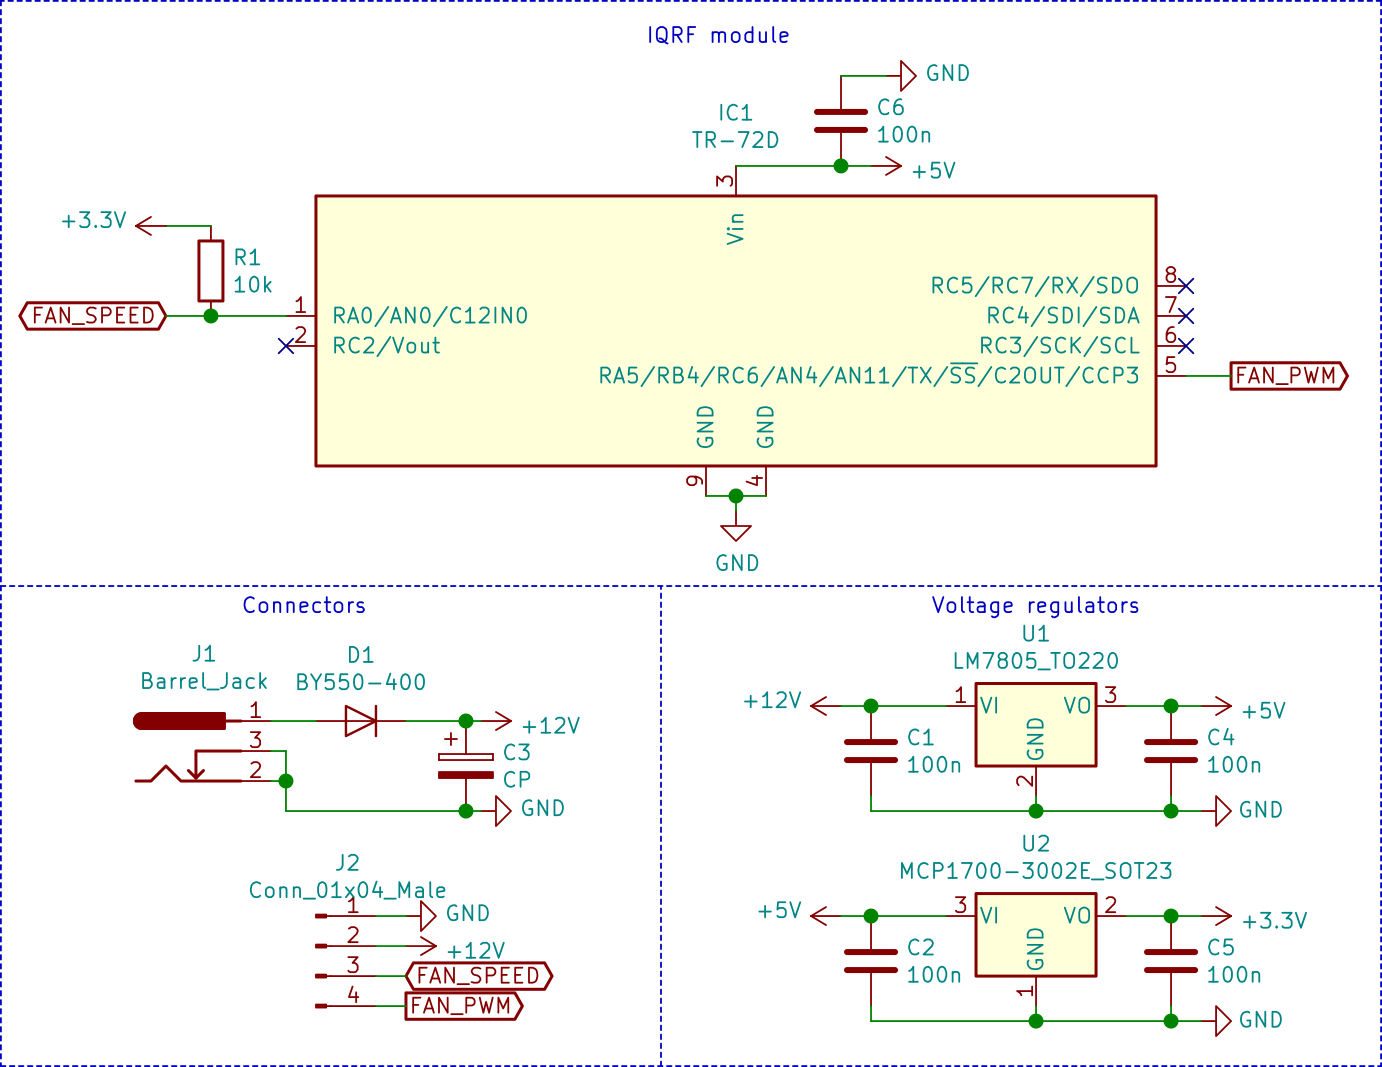
\includegraphics[width = 128mm]{img/kicad/fan-regulator-schema.png}
\caption{Obvodové schéma regulátoru}
\end{figure}

\begin{figure}[H]
\centering
\label{fig:board/fan-regulator}
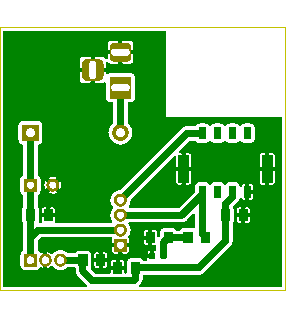
\includegraphics{img/kicad/fan-regulator-board.pdf}
\caption{Výkres plošného spoje regulátoru}
\end{figure}

\subsubsection{Bezdrátový modul IQRF TR-72DAT}

Pro komunikaci mezi bránou a regulátory jsem použil bezdrátový modul IQRF TR-72DAT, který rovněž vyrábí česká firma IQRF Tech s.r.o., která sídlí v~Jičíně. Plošný spoj modulu má podobné rozměry jako SIM\index[zkr]{SIM!Subscriber identity module|textit} karta, proto je pro jeho připojení s~deskou plošných spojů použit konektor pro SIM karty.

\begin{figure}[H]
\centering
\label{fig:iqrf/fotka}
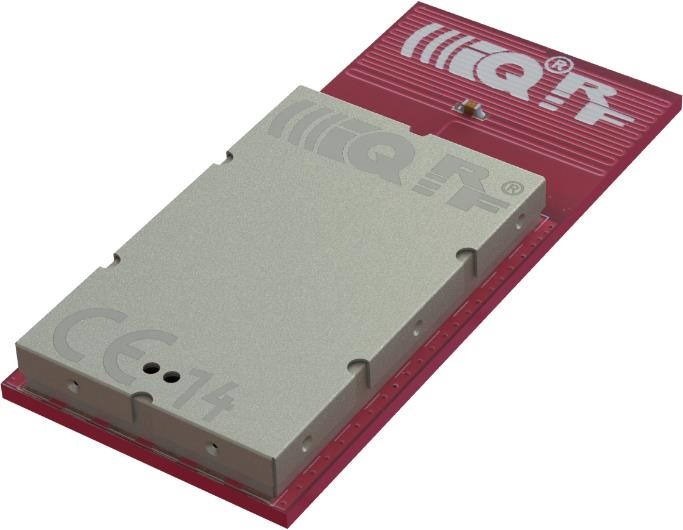
\includegraphics[width = 64mm]{img/iqrf/dctr-72dat.png}
\caption{Fotografie bezdrátového modulu IQRF TR-72DAT}
\end{figure}

Modul může vysílat na bezlicenčních pásmech 916~MHz, která je určené pro Ameriku, a 868~MHz, určené pro zbytek světa. Vysílací výkon modulu je 12,5~mW, používá GFSK\index[zkr]{GFSK!Gaussian frequency-shift keying|textit} modulaci. Modul má integrovanou anténu na svém plošném spoji.

Pro komunikaci používá tzv. mesh neboli smíšenou topologii. Ta má výhody v~robustnosti a v~absenci centrálního prvku. Její nevýhodou je naopak potřebná ochrana proti zacyklení a nutnost směrování provozu.

Modul lze napájet napětím 3,1~V až 5,5~V, protože obsahuje LDO\index[zkr]{LDO!Low-dropout|textit} napěťový stabilizátor Microchip MCP1700T-3002E/TT. Dále modul obsahuje mikrokontrolér Microchip PIC16LF1938. Ten užívá operační systém IQRF OS, který za uživatele zajišťuje komunikaci s~integrovaným obvodem STMicroelectronics Spirit1. Tento obvod řídí bezdrátový datový přenos a má hardwarovou podporu blokové šifry AES-128\index[zkr]{AES!Advanced Encryption Standard|textit}. Operační systém dále ovládá integrované periferie (například digitální teploměr). IQRF DPA\index[zkr]{DPA!Direct Peripheral Access|textit} a uživatelská aplikace. Dále modul obsahuje digitální teploměr Microchip MCP9808E/MC.

Microchip PIC16LF1938 je 8-bitový mikrokontrolér s~architekturou PIC\index[zkr]{PIC!Peripheral Interface Controller|textit}, která používá architekturu RISC\index[zkr]{RISC!Reduced instruction set computing|textit}, jenž má omezenou instruktážní sadu a rychlé vykonávání instrukcí. Flash paměť pro program má velikost 28~kB, paměť EEPROM má velikost 256~B a paměť SRAM\index[zkr]{SRAM!Static RAM|textit} má velikost 1~kB.

\begin{figure}[H]
\centering
\label{fig:iqrf/zjednodusene-schema}
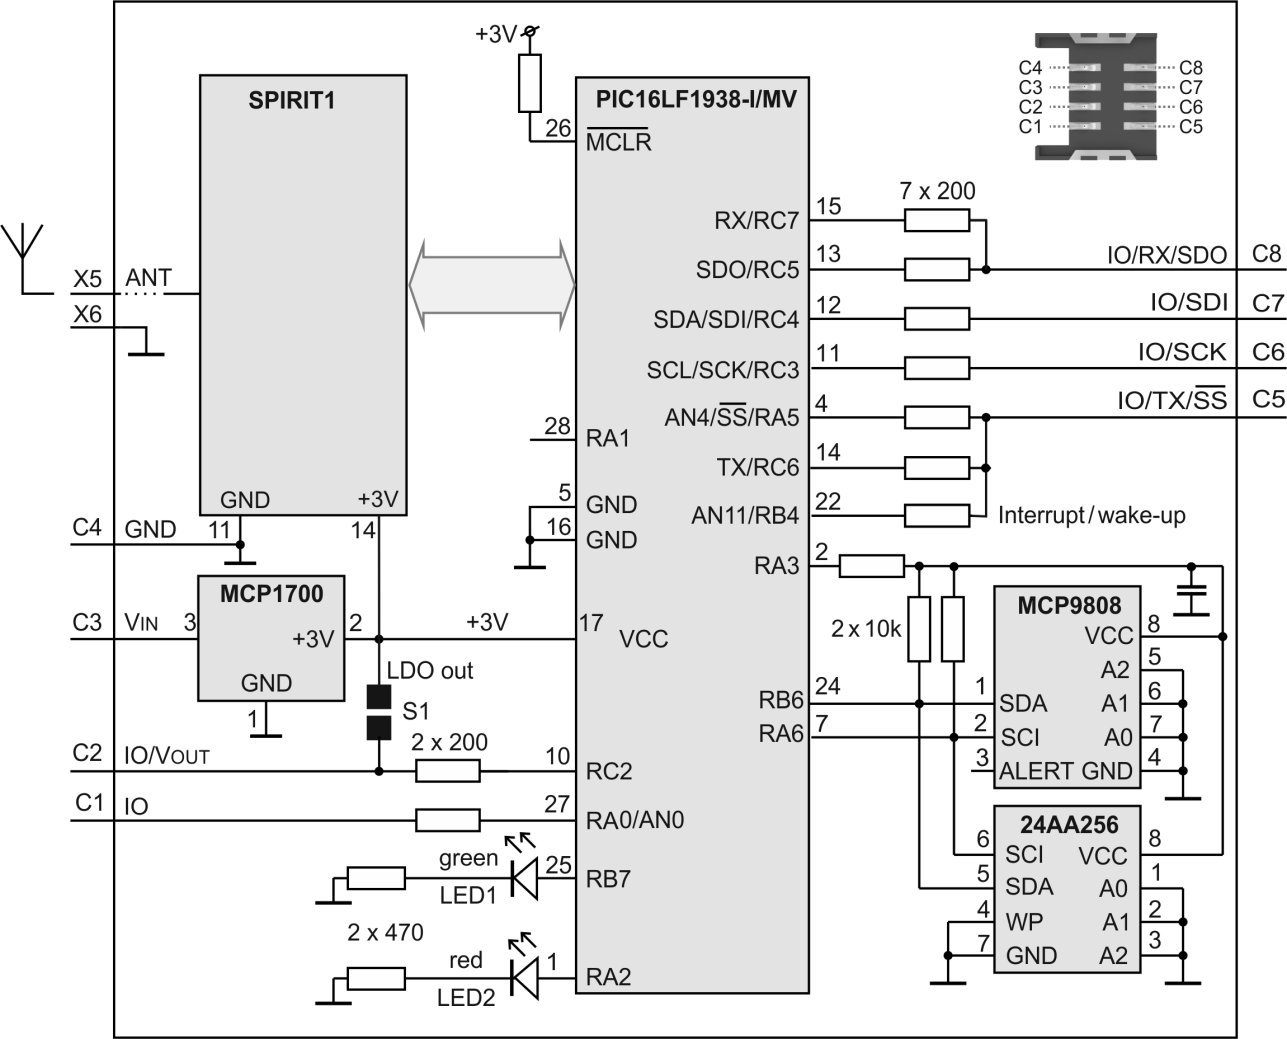
\includegraphics[width = 128mm]{img/iqrf/dctr-72dat-zjednodusene-schema.png}
\caption{Zjednodušené schéma bezdrátového modulu IQRF TR-72DAT}
\end{figure}

\newpage

\subsection{Senzor teploty a vlhkosti}

Pro svou funkčnost regulátor potřebuje 5~V napájecí spínaný zdroj, který dokáže dodat minimálně proud 1~A. Napětí 5~V je použito k~napájení samotného mikrokontroléru. Dále zařízení obsahuje 3,3~V lineární LDO napěťový regulátor AMS1117, který slouží pro napájení ethernetového řadiče a senzoru.

\begin{figure}[H]
\centering
\label{fig:schematic/sensor}
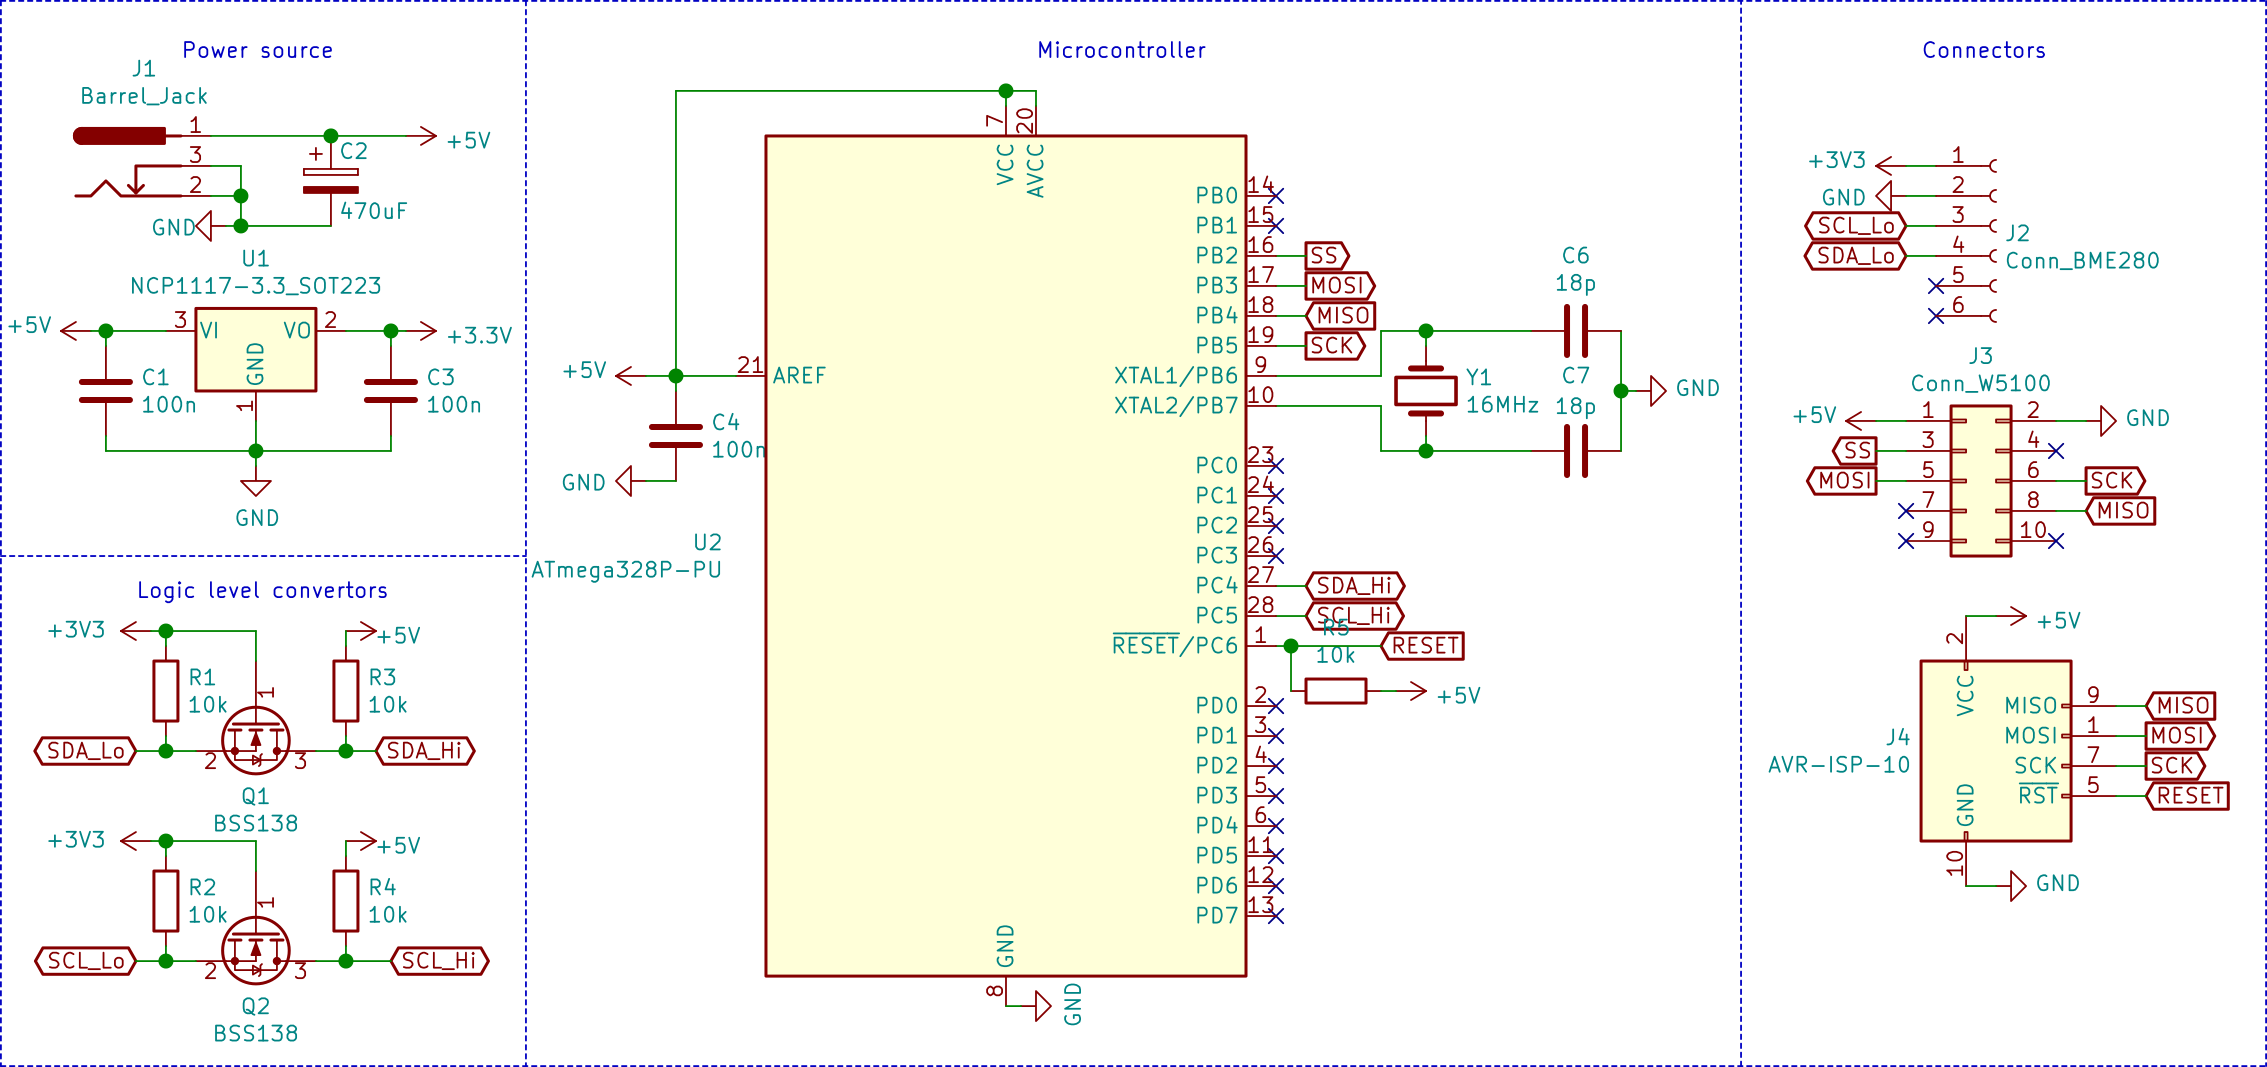
\includegraphics[width = 150mm]{img/kicad/sensor-schema.png}
\caption{Obvodové schéma senzoru teploty}
\end{figure}

\begin{figure}[H]
\centering
\label{fig:board/sensor}
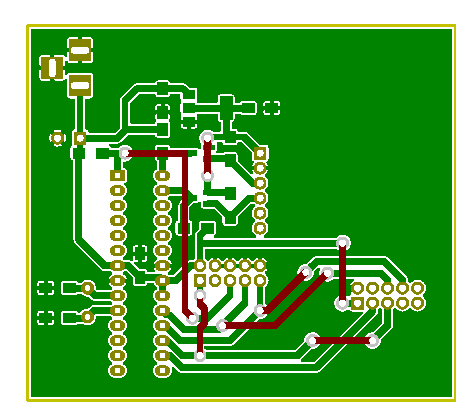
\includegraphics{img/kicad/sensor-board.pdf}
\caption{Výkres plošného spoje senzoru teploty}
\end{figure}

\newpage

\subsubsection{Mikrokontrolér Atmel ATmega328P}

Jako řídící mikrokontrolér jsem zvolil Atmel ATmega328P, který běží na frekvenci 16 MHz. Jedná se o~8‑bitový mikrokontrolér s~architekturou AVR\index[zkr]{AVR!Alf and Vegard's RISC processor|textit}, která používá architekturu RISC, jenž má omezenou instruktážní sadu a rychlé vykonávání instrukcí. Flash paměť pro program má velikost 32~kB, paměť EEPROM má velikost 1~kB a paměť SRAM má velikost 2~kB. Má 23 programovatelných vstupních a výstupních pinů. Některé piny jsou určeny pro speciální použití jako je A/D převodník, analogový komparátor, UART, SPI, I$^{2}$C\index[zkr]{I$^{2}$C!Inter-Integrated Circuit|textit}, PWM, časovač/čítač nebo přerušení (IRQ\index[zkr]{IRQ!Interrupt ReQuest|textit}).

\begin{figure}[H]
\centering
\label{fig:atmega328p-block-diagram}
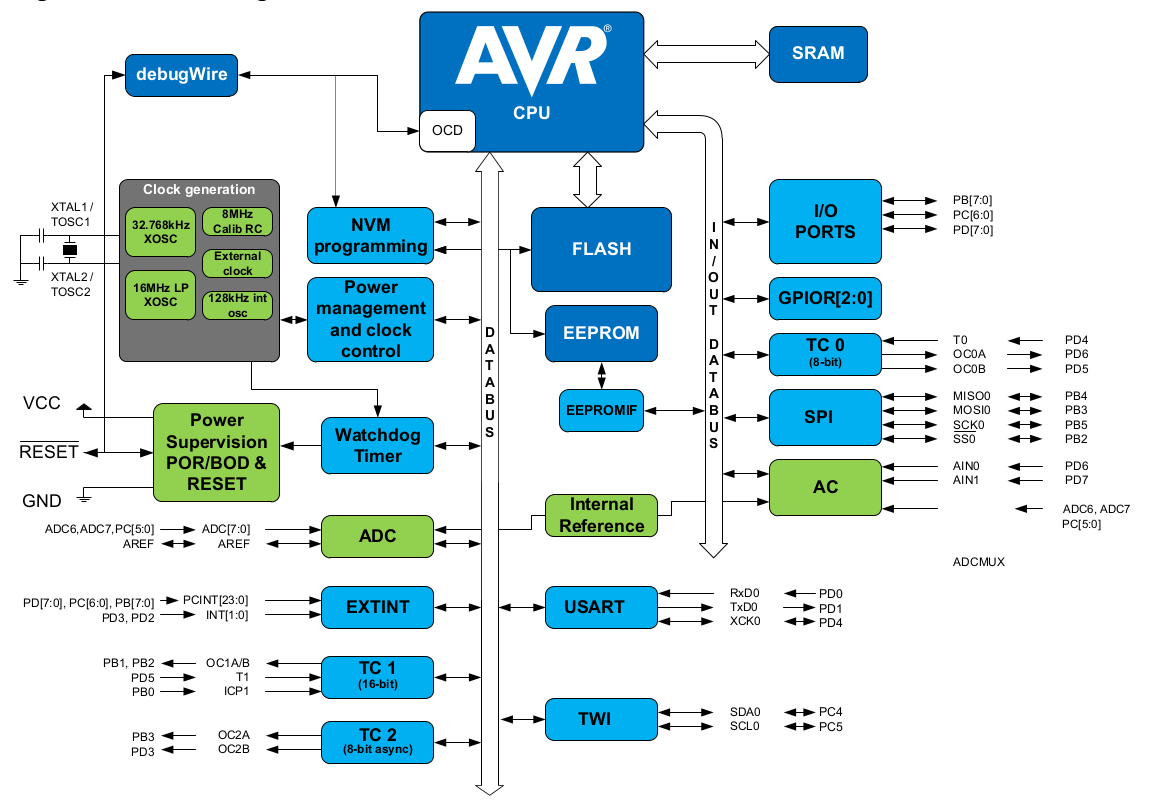
\includegraphics[width = 128mm]{img/atmega328p-block-diagram.png}
\caption{Blokové schéma mikrokontroléru ATmega328P}
\end{figure}

\begin{figure}[H]
\centering
\label{fig:atmega328p-pinout}
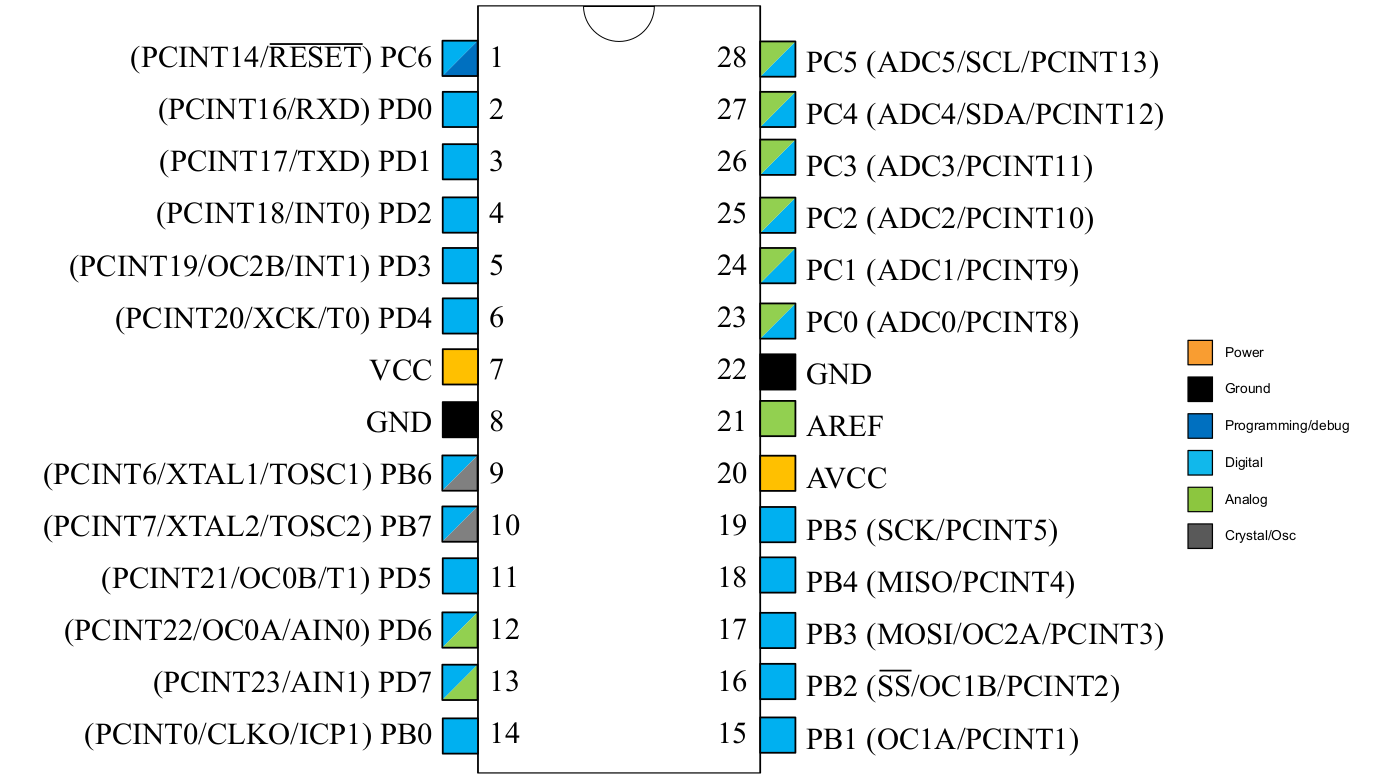
\includegraphics[width = 128mm]{img/atmega328p-pinout.png}
\caption{Popis vývodů mikrokontroléru ATmega328P v~pouzdru DIP-28}
\end{figure}

\newpage

\subsubsection{Ethernetový řadič WIZnet W5100}

Pro komunikaci mezi bránou a senzorem je použit Ethernet. Protože samotný mikrokontrolér neobsahuje řadič pro komunikaci přes Ethernet, je použit externí řadič WIZnet 5100. Tento řadič komunikuje s~mikrokontrolérem po sběrnici SPI. Řadič obsahuje hardwarovou implementaci protokolů IPv4\index[zkr]{IPv4!Internet Protocol version 4|textit}, ICMP\index[zkr]{ICMP!Internet Control Message Protocol|textit}, TCP\index[zkr]{TCP!Transmission Control Protocol|textit} a UDP\index[zkr]{UDP!User Datagram Protocol|textit}. Řadič je napájen 3,3~V a je kompatibilní s~5~V logickou úrovní mikrokontroléru. Protože řadič je vyráběn pouze v pouzdře LQFP-80, které je téměř nemožné v domácích podmínkách osadit, je použit hotový modul.

\begin{figure}[H]
\centering
\label{fig:w5100-block-diagram}
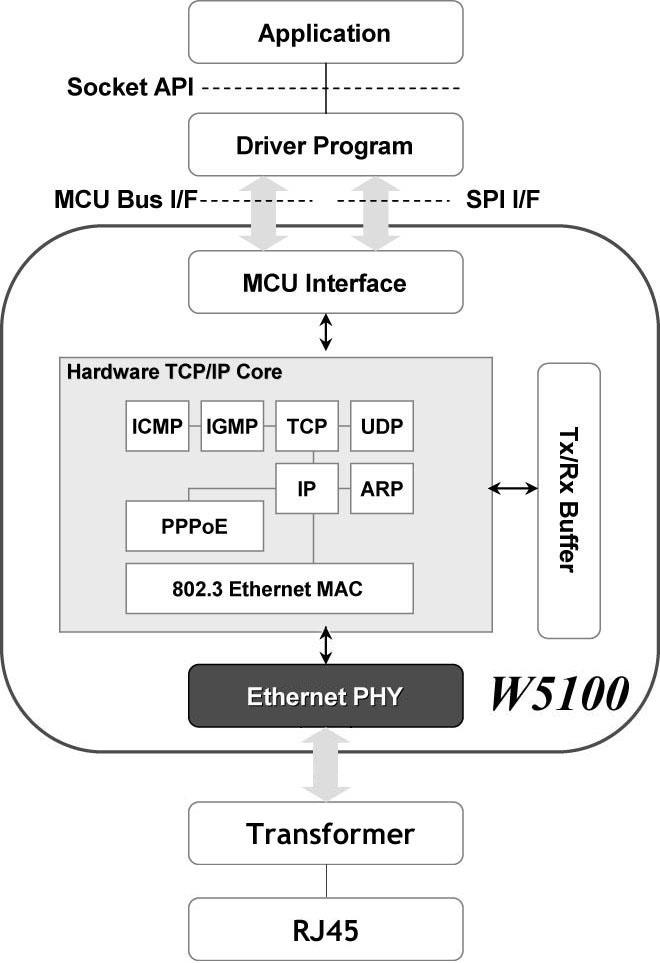
\includegraphics[width = 96mm]{img/w5100-block-diagram.png}
\caption{Blokové schéma ethernetového řadiče WIZnet W5100}
\end{figure}

\newpage

\subsubsection{Senzor Bosch BME280}

Jako senzor teploty jsem zvolil Bosch BME280, který kromě teploty měří také relativní vlhkost a atmosferický tlak. Mikrokontrolér může se senzorem komunikovat po sběrnici I$^{2}$C nebo SPI. Zvolil jsem komunikaci po sběrnici I$^{2}$C, protože po sběrnici SPI již komunikuje ethernetový řadič. Senzor je napájen 3,3~V a je kompatibilní pouze s~3,3~V logickou úrovní, proto musí být použit převodník logických úrovních, který se skládá z~N-MOSFET tranzistoru BSS138 a dvou pull-up resistorů. Protože senzor je vyráběn pouze v LGA pouzdře, které je téměř nemožné v domácích podmínkách osadit, je použit hotový modul.

\begin{figure}[H]
\centering
\label{fig:bme280-block-diagram}
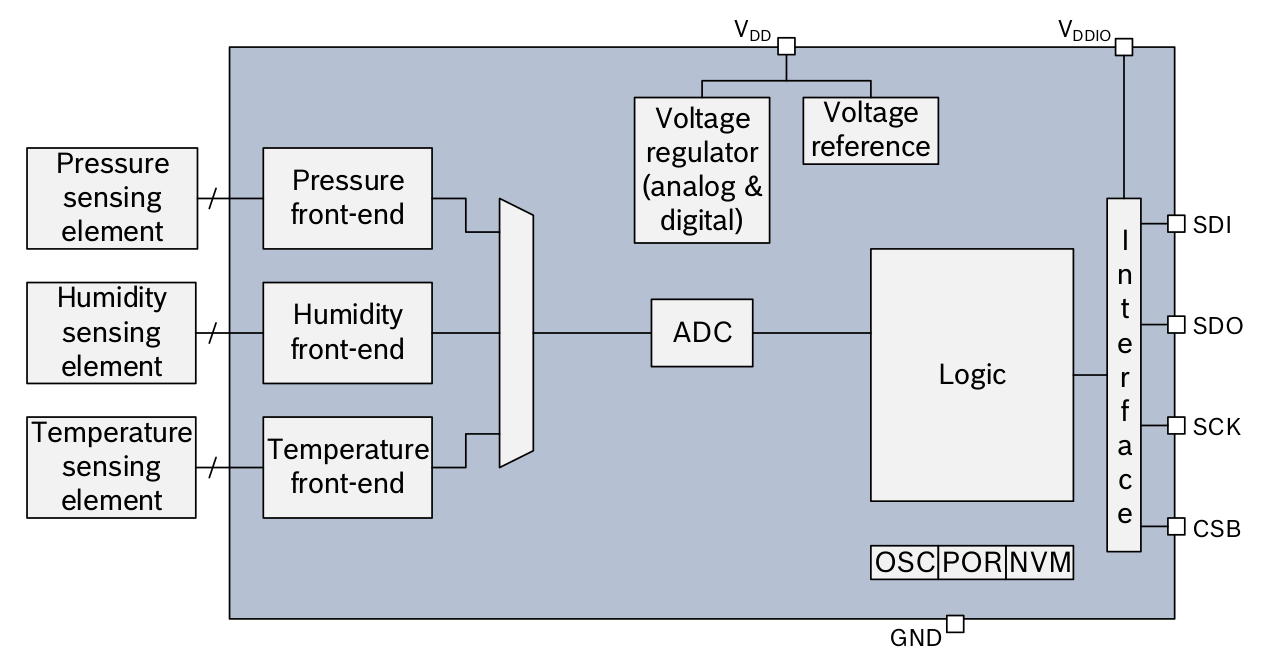
\includegraphics[width = 128mm]{img/bme280-block-diagram.png}
\caption{Blokové schéma senzoru Bosch BME280}
\end{figure}

\newpage

\subsection{Brána}

Jako bránu jsem použil jednodeskový počítač Raspberry Pi 3 model B. Bezdrátový modul IQRF TR-72DAT je k~bráně připojen přes sběrnici SPI\index[zkr]{SPI!Serial Peripheral Interface|textit} pomocí adaptéru IQRF KON-RASP-01. Brána se napájí pomocí externího spínaného zdroje s~microUSB konektorem, který má výstupní napětí 5~V a maximální výstupní proud 2~A.

\subsubsection{Raspberry Pi 3 model B}

Raspberry Pi 3 model B je jednodeskový počítač, který má rozměry podobné kreditní kartě. Tento počítač obsahuje:

\begin{itemize}
  \item čtyřjádrový ARM\index[zkr]{ARM!Acorn RISC Machine|textit}\index[zkr]{ARM!Advanced RISC Machine|textit} Cortex-A53 Broadcom BCM2837,
  \item 1~GB operační paměti RAM\index[zkr]{RAM!Random-access memory|textit},
  \item čtyři USB 2.0 porty
  \item port RJ45 pro 100~Mb síťovou kartu,
  \item slot pro microSD\index[zkr]{SD!Secure Digital|textit} kartu,
  \item HDMI\index[zkr]{HDMI!High-Definition Multimedia Interface|textit} výstup,
  \item 40 GPIO\index[zkr]{GPIO!General-purpose input/output|textit} pinů, na kterých jsou vyvedeny sběrnice SPI\index[zkr]{SPI!Serial Peripheral Interface|textit}, I$^{2}$C, USART\index[zkr]{USART!Universal Synchronous / Asynchronous Receiver and Transmitter|textit}.
\end{itemize}

\begin{figure}[H]
\centering
\label{fig:foto/rpi3}
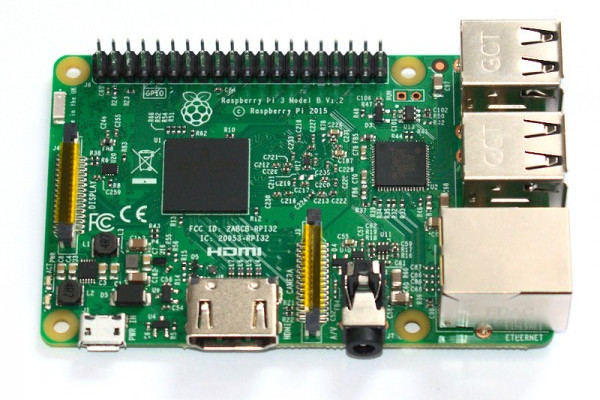
\includegraphics[width = 128mm]{img/foto/rpi3.jpg}
\caption{Fotografie jednodeskového počítače Raspberry Pi 3 model B}
\end{figure}

\newpage

\section{Návrh software}

\subsection{Komunikace}

Pro komunikaci mezi jednotlivými uzly sítě IQRF je použit protokol IQMESH, ve kterém jsou data šifrována. Pro komunikaci regulátoru s~bránou jsem použil protokol MQTT\index[zkr]{MQTT!Message Queuing Telemetry Transport|textit}.

\subsection{PWM regulátor ventilátoru}

Software regulátoru je napsán v C++ s použitím platformy Arduino. Největší výhodou této platformy je velká uživatelská základna a dostupnost knihoven pro různé periferie. Software byl napsán ve vývojovém prostředí PlatformIO IDE\cite{sw/platformio-ide}\index[zkr]{IDE!Integrated Development Environment|textit}, které je založeno na textovém editoru Atom\cite{sw/atom} a řeší za uživatele stažení knihoven, na kterých projekt závisí.

\subsubsection{Vývojové prostředí PlatformIO IDE}

Vývojové prostředí PlatformIO IDE je založeno na open-source textovém editoru Atom, který je vyvíjen společností GitHub. Tento editor je rozšířen o~nástroje pro vývoj aplikací pro embedded zařízení (např. Arduino, ESP32). PlatformIO je open-source nástroj, který se stará o závislosti jednotlivých projektů a knihoven. Tento nástroj je napsán ve~skriptovacím jazyce Python. 

\begin{figure}[H]
\centering
\label{fig:platformio-ide}
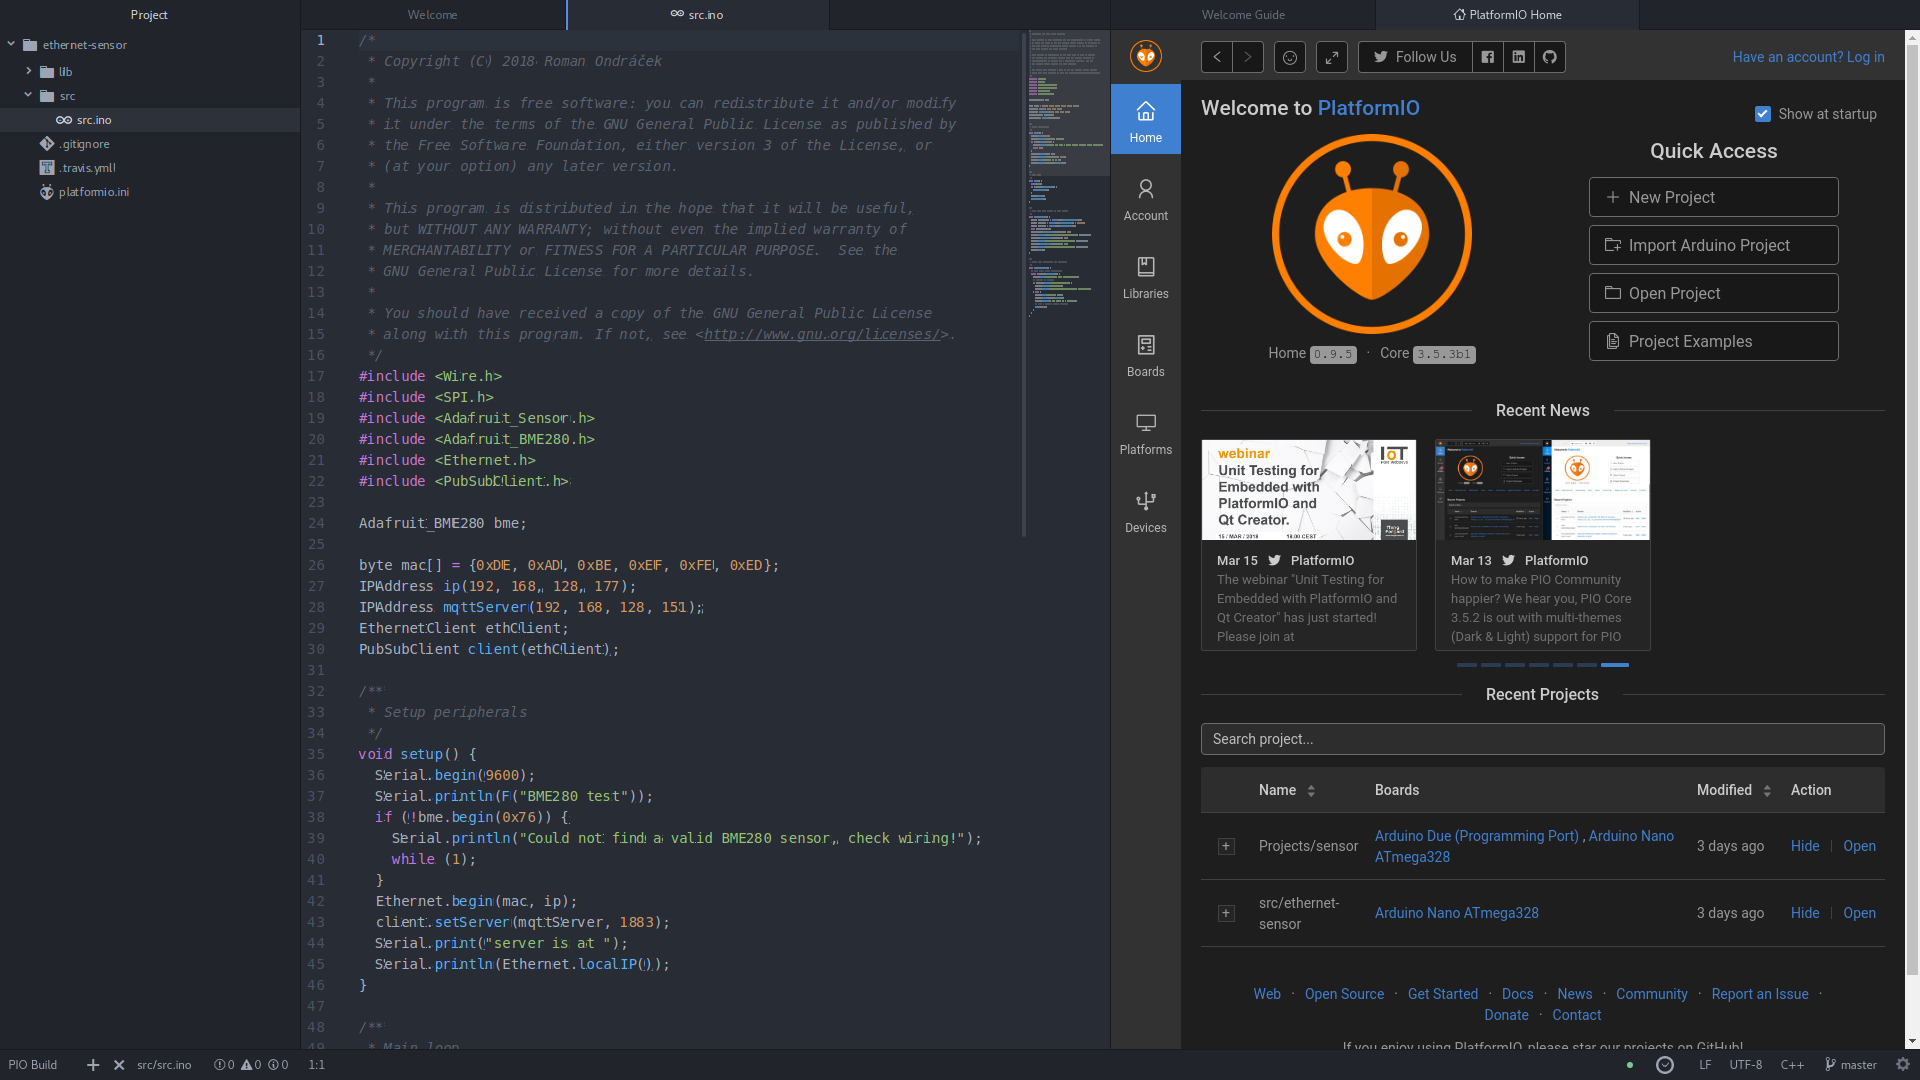
\includegraphics[width = 150mm]{img/platformio-ide.png}
\caption{Vývojové prostředí PlatformIO IDE}
\end{figure}

\newpage

\subsection{Senzor teploty a vlhkosti}

Software senzoru je napsán v~programovacím jazyce C. Software byl napsán ve vývojovém prostředí IQRF IDE\cite{iqrf/ide}.

\subsubsection{Vývojové prostředí IQRF IDE}

IQRF IDE\cite{iqrf/ide} je zdarma stažitelné vývojové prostředí, které je určené pro vývoj aplikací pro bezdrátové moduly IQRF. Toto vývojové prostředí je pouze pro operační systém Microsoft Windows. Uživatelé operačního systému Apple OS X nebo libovolné linuxové distribuce nemohou vyvíjet software pro tyto bezdrátové moduly. IQRF IDE používá kompilátor CC5X C Compiler\cite{sw/cc5x-compiler}.

\begin{figure}[H]
\centering
\label{fig:iqrf/ide}
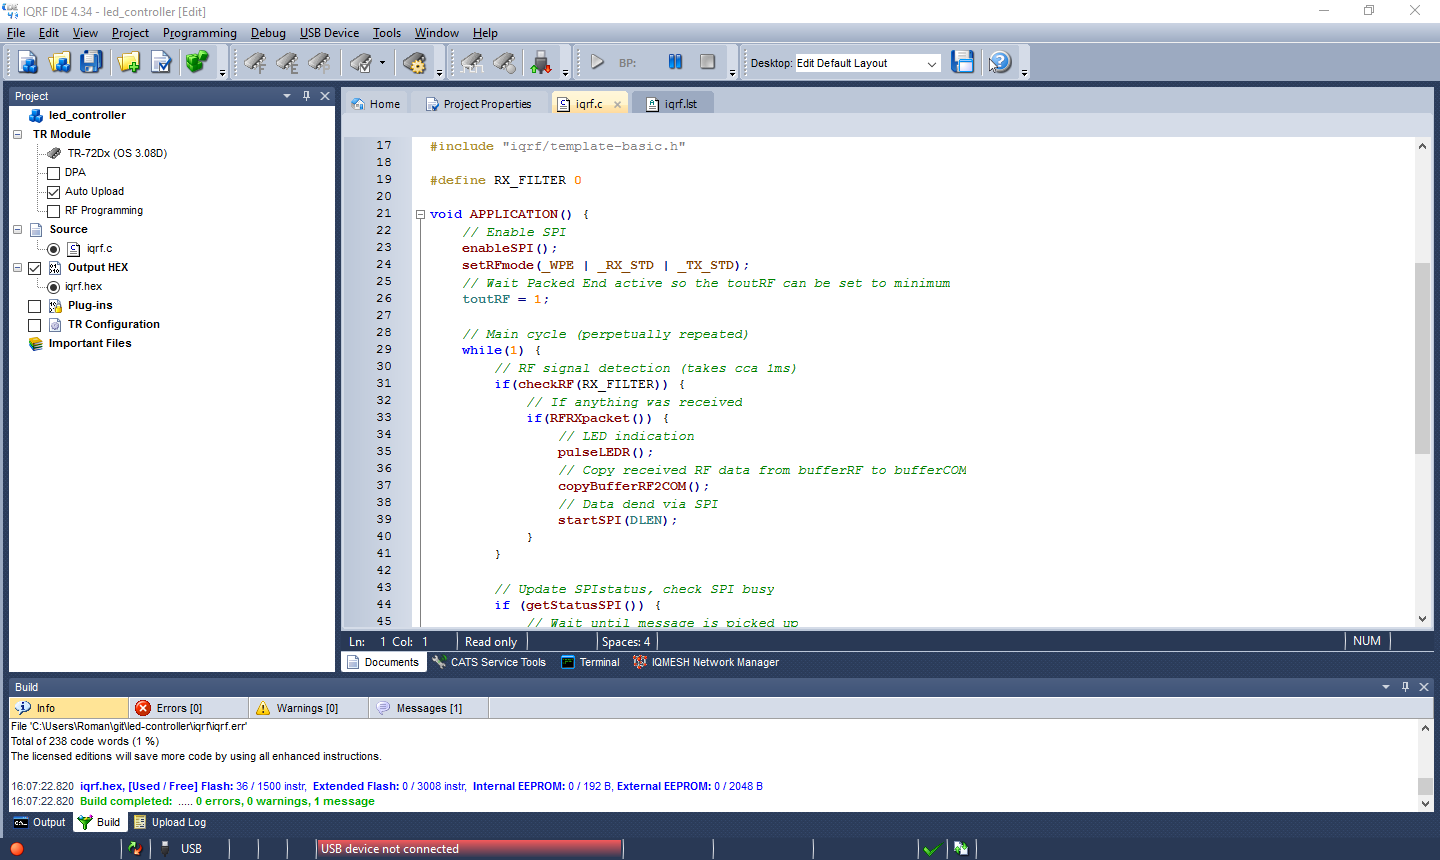
\includegraphics[width = 150mm]{img/iqrf/ide.png}
\caption{Vývojové prostředí IQRF IDE}
\end{figure}

\newpage

\subsubsection{Operační systém IQRF OS}

IQRF OS\cite{iqrf/os} je operační systém určený pro bezdrátové moduly IQRF, pomocí kterého může uživatel jednoduše:

\begin{itemize}
  \item ovládat rádiovou komunikaci,
  \item ovládat komunikaci v~mesh síti,
  \item komunikovat s~periferiemi přes sběrnice SPI, USART, I$^{2}$C,
  \item pracovat s~pamětmi RAM\index[zkr]{RAM!Random-access memory|textit}, EEPROM\index[zkr]{EEPROM!Electrically Erasable Programmable Read-Only Memory|textit},
  \item inicializovat GPIO,
  \item spínat GPIO,
  \item číst logické hodnoty z~GPIO,
  \item spínat integrované LED\index[zkr]{LED!Light-Emitting Diode|textit} diody,
  \item generovat PWM\index[zkr]{PWM!Pulse Width Modulation|textit} na výstupním pinu,
  \item číst hodnoty z~analogově digitálního převodníku,
  \item číst teplotu z~integrovaného teplotního senzoru.
\end{itemize}

\begin{figure}[H]
\centering
\label{fig:foto/iqrf-os}
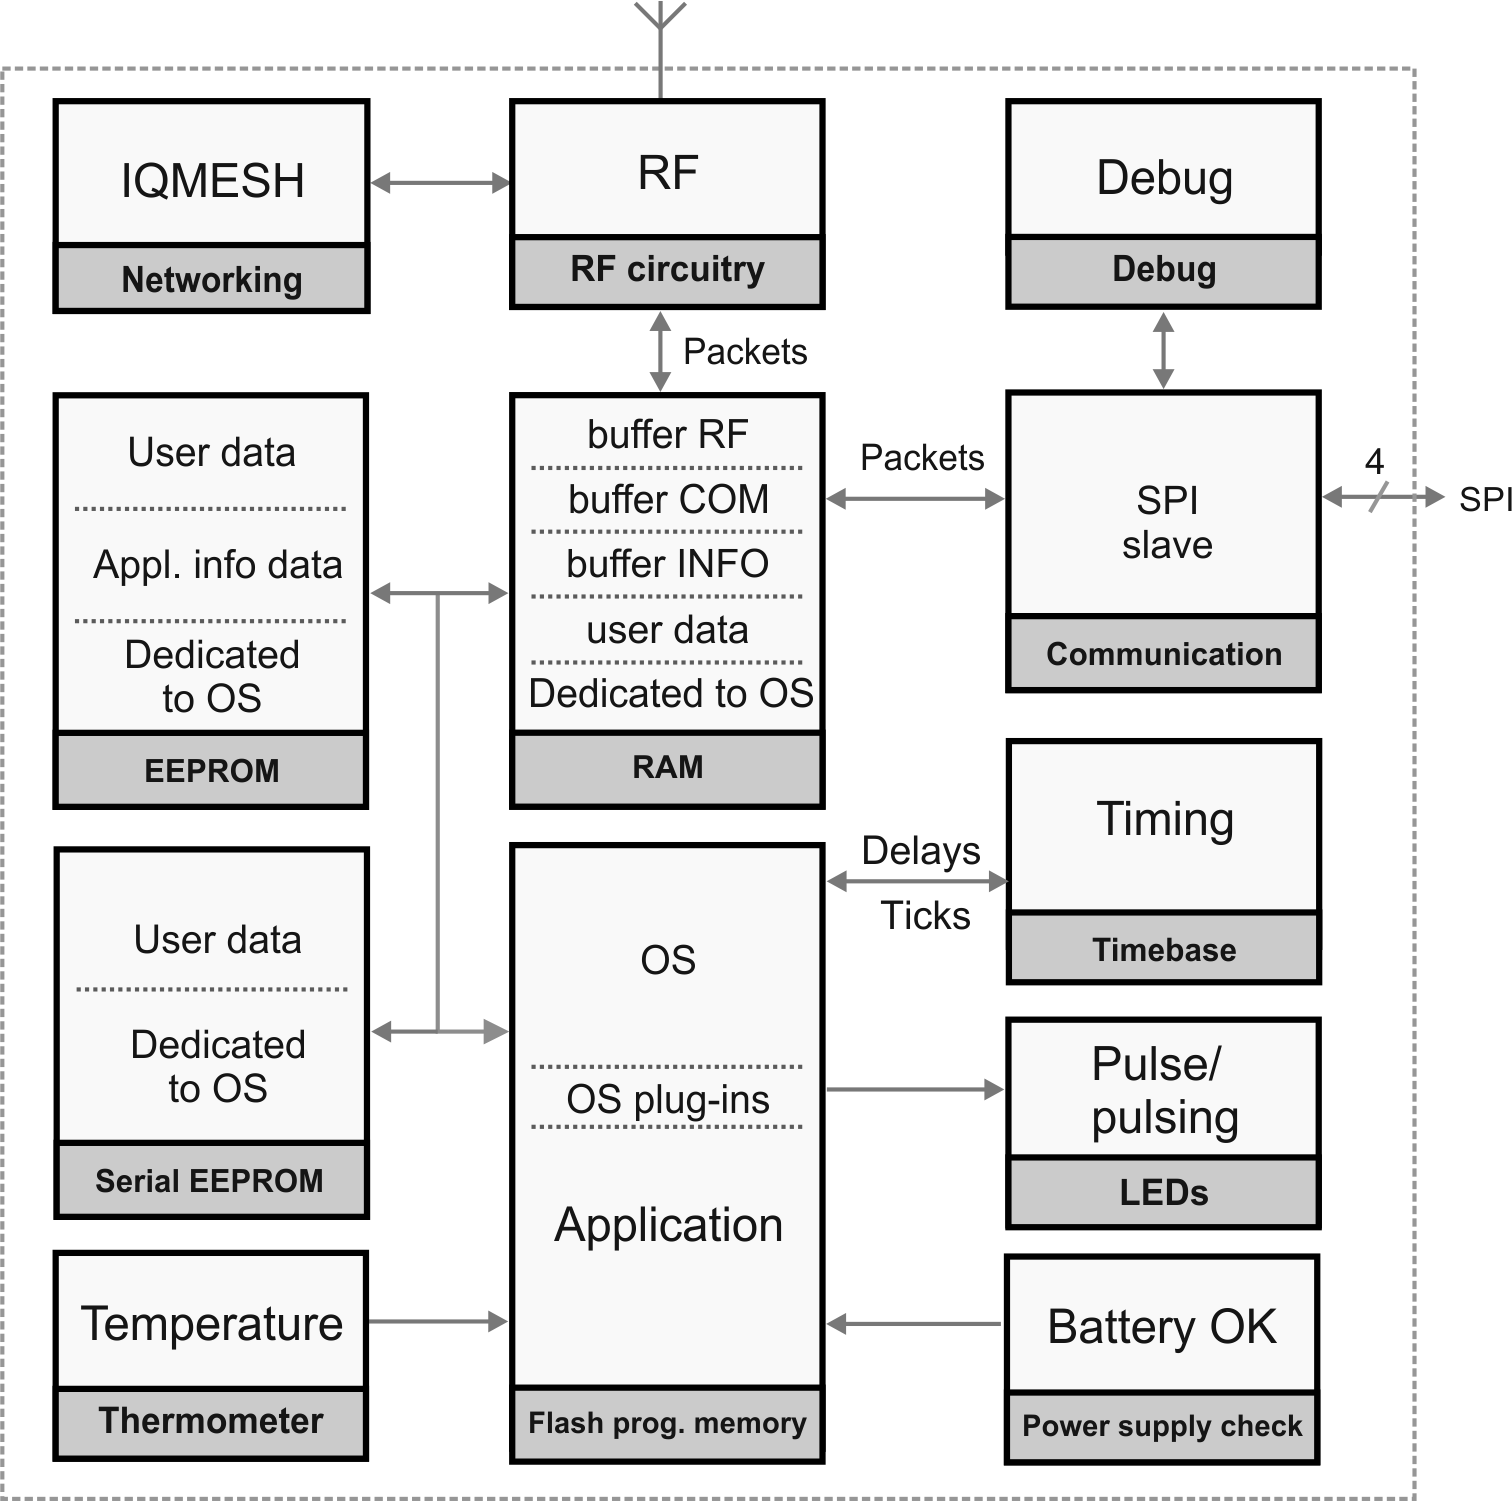
\includegraphics[width = 100mm]{img/iqrf/os-blokove-schema.png}
\caption{Blokové schéma operačního systému IQRF OS}
\end{figure}

\newpage

\subsubsection{Protokol IQRF DPA}

IQRF DPA\cite{iqrf/dpa} je vrstva nad IQRF OS, která se stará o~protokol komunikace IQRF bezdrátových modulů. IQRF DPA má pevně danou strukturu paketů, která je uvedena v~tabulce č.~1. Centrální prvek v~IQRF mesh síti se jmenuje koordinátor, který je umístěn v~bráně. Koordinátor má se své paměti EEPROM uložené informace o~dalších bezdrátových modulech, se kterými má komunikovat. Pokud koordinátor přijme data od bezdrátového modulu, jehož informace nemá uložené v~EEPROM paměti, pak data ignoruje. Při vytváření sítě se ve vývojovém prostředí nastavují symetrické šifrovací klíče pro šifrování komunikace pomocí symetrické šifry AES-128.

Paket pro nastavení střídy PWM signálu o frekvenci 1~kHz je uveden v~tabulce č.~2 a paket pro vyčtení hodnoty z analogově digitálního převodníku je uveden v~tabulce č.~3.

\begin{table}[H]
\centering
\begin{tabular}{|c|c|c|c|c|}
\hline
NADR & PNUM & PCMD & HWPID & DATA \\
\hline
siťová adresa & číslo periferie & příkaz & HWP\index[zkr]{HWP!Hardware profile|textit} identifikátor & data \\
\hline
\end{tabular}
\caption{Schéma paketu IQRF DPA}\label{table:iqrf/dpa}
\end{table}

\begin{table}[H]
\centering
\begin{tabular}{|c|c|c|c|c|c|c|}
\hline
NADR & PNUM & PCMD & HWPID & Prescaler & Period & Duty \\
\hline
0x04 & 0x20 & 0x00 & 0xFFFF & 0x02 & 0x7D & střída \\
\hline
\end{tabular}
\caption{Schéma paketu pro nastavení střídy (0x00-0x80) PWM signálu}\label{table:iqrf/dpa-pwm}
\end{table}

\begin{table}[H]
\centering
\begin{tabular}{|c|c|c|c|}
\hline
NADR & PNUM & PCMD & HWPID \\
\hline
0x04 & 0x21 & 0x00 & 0xFF \\
\hline
\end{tabular}
\caption{Schéma paketu pro vyčtení hodnoty z ADC\index[zkr]{ADC!Analog-to-digital converter|textit}\index[zkr]{ADC!Analogově digitální převodník|textit}}\label{table:iqrf/dpa-adc}
\end{table}

\newpage

\subsection{Brána}

V~bráně běží linuxová distribuce Raspbian, což je speciálně upravená linuxová distribuce pro jednodeskový počítač Raspberry Pi. Tato linuxová distribuce je odvozená od linuxové distribuce Debian, která je jedna z~nejpoužívanějších linuxových distribucích.

\subsubsection{IQRF Gateway Daemon}

Pro komunikaci s~IQRF sítí je použit IQRF Gateway Daemon\cite{iqrfsdk/iqrf-daemon}, což je open source software pod licencí Apache License 2.0 vyvíjený firmou IQRF Tech s.r.o., který obstarává komunikaci mezi IQRF sítí a MQTT brokerem. Tento software je napsán v~programovavím jazyku C++. Konfigurační soubory jsou psány ve~formátu JSON\index[zkr]{JSON!JavaScript Object Notation|textit}.

Pro uživatelsky přívětivou konfiguraci IQRF Gateway Daemonu jsem vytvořil webovou aplikaci\cite{iqrfsdk/iqrf-daemon-webapp}, která je napsaná ve skriptovacím jazyce PHP s~použitím českého frameworku Nette\cite{nette}.

\begin{figure}[H]
\centering
\label{fig:iqrf/iqrf-daemon-webapp}
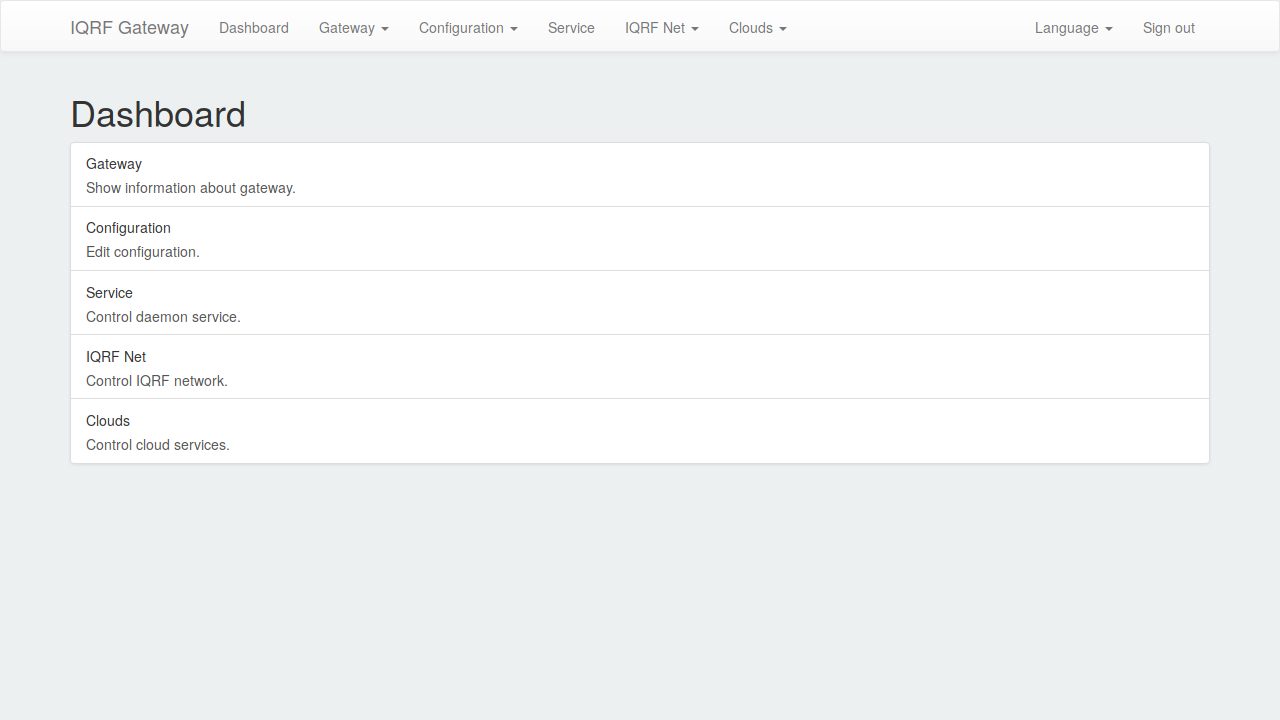
\includegraphics[width = 150mm]{img/iqrf/iqrf-daemon-webapp.png}
\caption{Výchozí stránka IQRF Gateway Daemon webapp}
\end{figure}

\subsubsection{MQTT boker mosquitto}

Jako MQTT broker jsem pouřil open-source software mosquitto\cite{sw/mosquitto}, který je vyvíjen společností Eclipse v programovacím jazyce C. Obsahuje klientskou i serverovou část. Implementuje standardy MQTT 3.1 a MQTT 3.1.1.

\newpage

\subsubsection{Node-RED}

Pro zpracování a vizualizaci dat jsem zvolil nástroj Node-RED\cite{sw/node-red}, což je open-source software původně vyvíjený společností IBM, který má za úkol usnadnění připojení zařízení do Internetu - tzv. IoT. Tento nástroj je napsán v skriptovacím jazyce JavaScript s~použitím frameworku Node.js.

Program vytvořený v Node-REDu se skládá z~bloků, které jsou rozděleny na vstupní bloky, výstupní bloky, funkční bloky, atd.

\begin{figure}[H]
\centering
\label{fig:node-red}
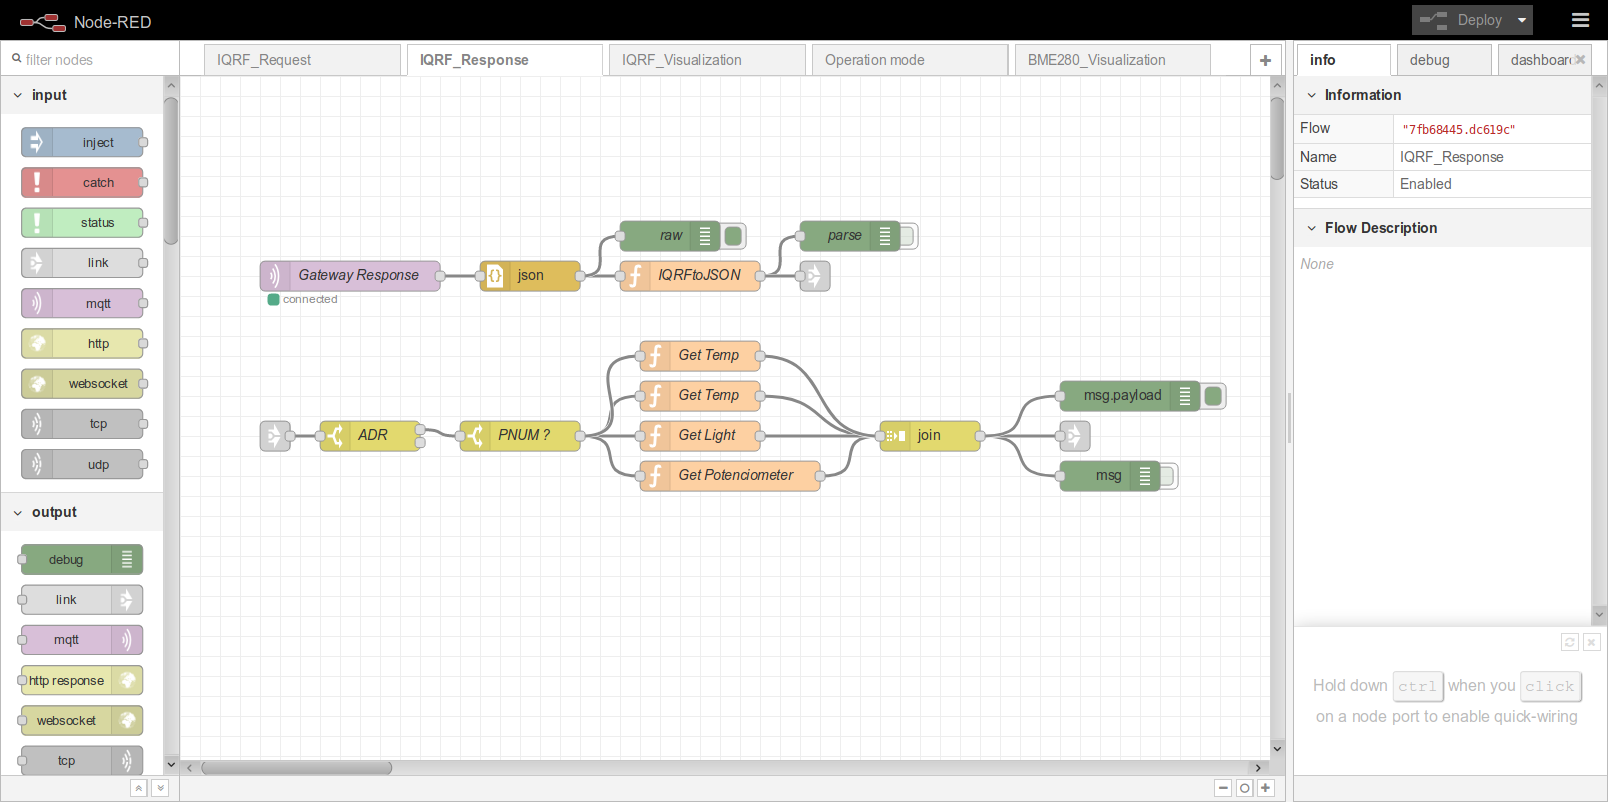
\includegraphics[width = 150mm]{img/node-red.png}
\caption{Webové vývojové prodtředí Node-REDu}
\end{figure}

\begin{figure}[H]
\centering
\label{fig:node-red_dashboard}
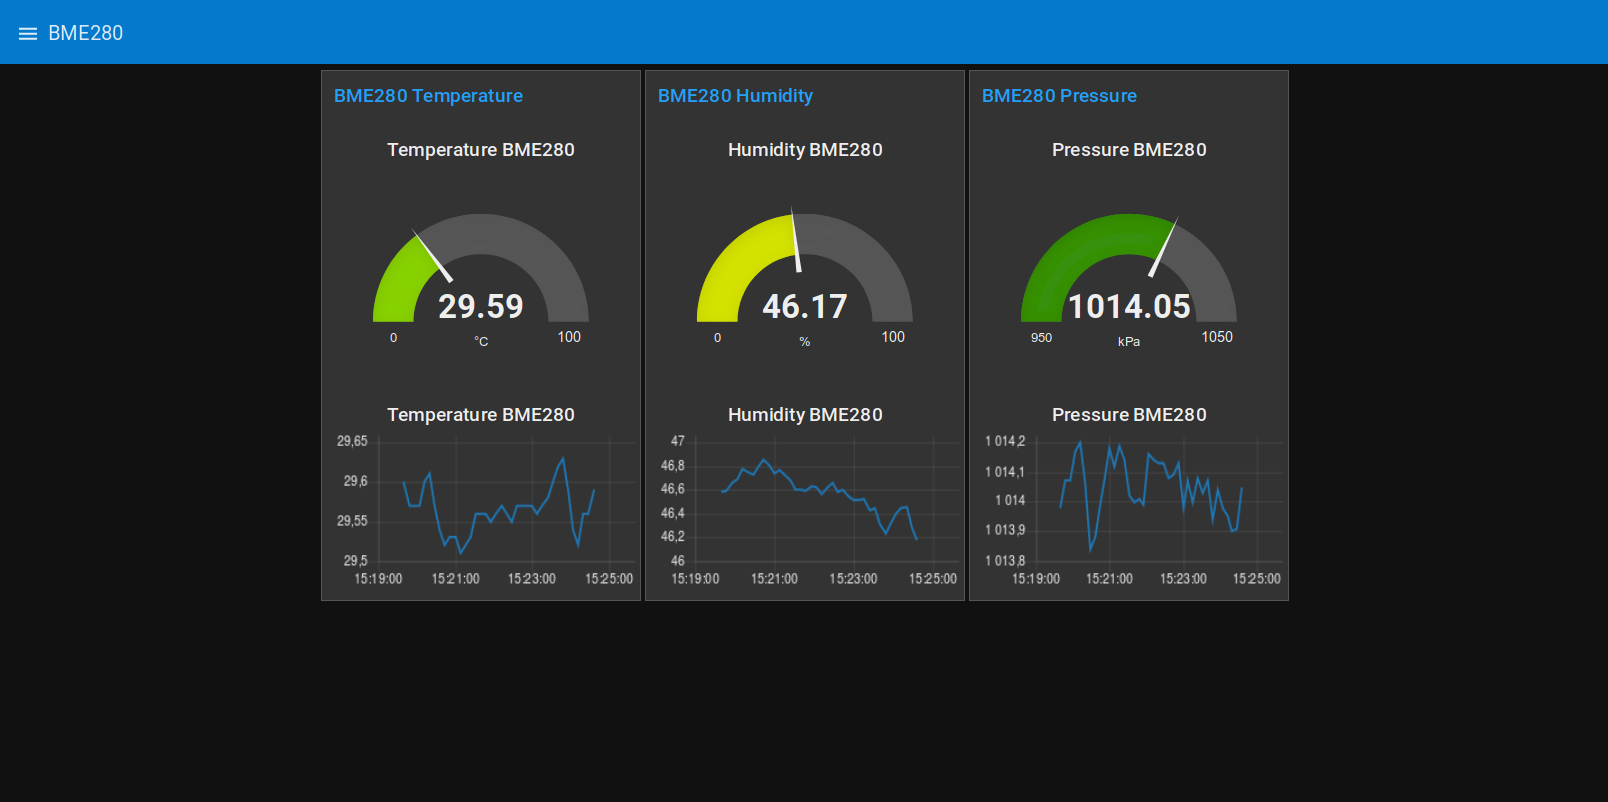
\includegraphics[width = 150mm]{img/node-red_dashboard.png}
\caption{Node-RED Dashboard s grafy}
\end{figure}

\newpage

\section{Technické parametry}

\subsection{PWM regulátor}

\begin{table}[H]
  \centering
  \begin{tabular}{lr}
    \hline
    \textbf{Technické parametry} & ~ \\
    \hline
    \hline
    \textbf{Rozměry} & 4,8$\times$4,8$\times$3~cm \\
    \hline
    \textbf{Elektrické parametry} \\
    \hline
    \hline
    \textbf{Napájecí napětí} & 12~V DC\index[zkr]{DC!Direct current|textit} \\
    \textbf{Typická spotřeba} & méně než 0,5~W \\
    \textbf{Maximální spínatelný proud} & 1~A \\
    \hline
    \textbf{Ostatní parametry} \\
    \hline
    \hline
    \textbf{Přenos dat} & bezdrátově na frekvenci 868~MHz \\
    \textbf{Protokol} & IQRF DPA \\
  \end{tabular}
  \caption{Parametry PWM regulátoru}\label{table:parametry/fan-regulator}
\end{table}

\subsection{Senzor teploty}

\begin{table}[H]
  \centering
  \begin{tabular}{lr}
    \hline
    \textbf{Technické parametry} & ~ \\
    \hline
    \hline
    \textbf{Rozměry} & 4,8$\times$4,8$\times$3~cm \\
    \hline
    \textbf{Elektrické parametry} \\
    \hline
    \hline
    \textbf{Napájecí napětí} & 5~V DC\index[zkr]{DC!Direct current|textit} \\
    \textbf{Typická spotřeba} & méně než 2~W \\
    \hline
    \textbf{Ostatní parametry} \\
    \hline
    \hline
    \textbf{Přenos dat} & 10~Mb Ethernet \\
    \textbf{Protokol} & MQTT \\
  \end{tabular}
  \caption{Parametry senzoru teploty}\label{table:parametry/senzor}
\end{table}

\subsection{Brána}

\begin{table}[H]
  \centering
  \begin{tabular}{lr}
    \hline
    \textbf{Technické parametry} & ~ \\
    \hline
    \hline
    \textbf{Rozměry} & 7$\times$12$\times$4,5~cm \\
    \hline
    \textbf{Elektrické parametry} \\
    \hline
    \hline
    \textbf{Napájecí napětí} & 5~V DC \\
    \textbf{Typická spotřeba} & 6~W \\
  \end{tabular}
  \caption{Parametry brány}\label{table:parametry/zbrana}
\end{table}

\newpage

\section*{Závěr}

\addcontentsline{toc}{section}{Závěr}

Navržený systém měření a regulace teploty v~domácnosti byl navržen a realizován ve formě funkčního vzorku. Na obrázcích č.~18, č.~19 a č.~20 jsou fotografie funkčních vzorků brány, PWM regulátoru ventilátoru a senzoru. Vzhledem k~charakteru a univerzalitě řešení systém lze v~budoucnosti rozšířit o~další zařízení.

\begin{figure}[H]
\centering
\label{fig:foto/brana}
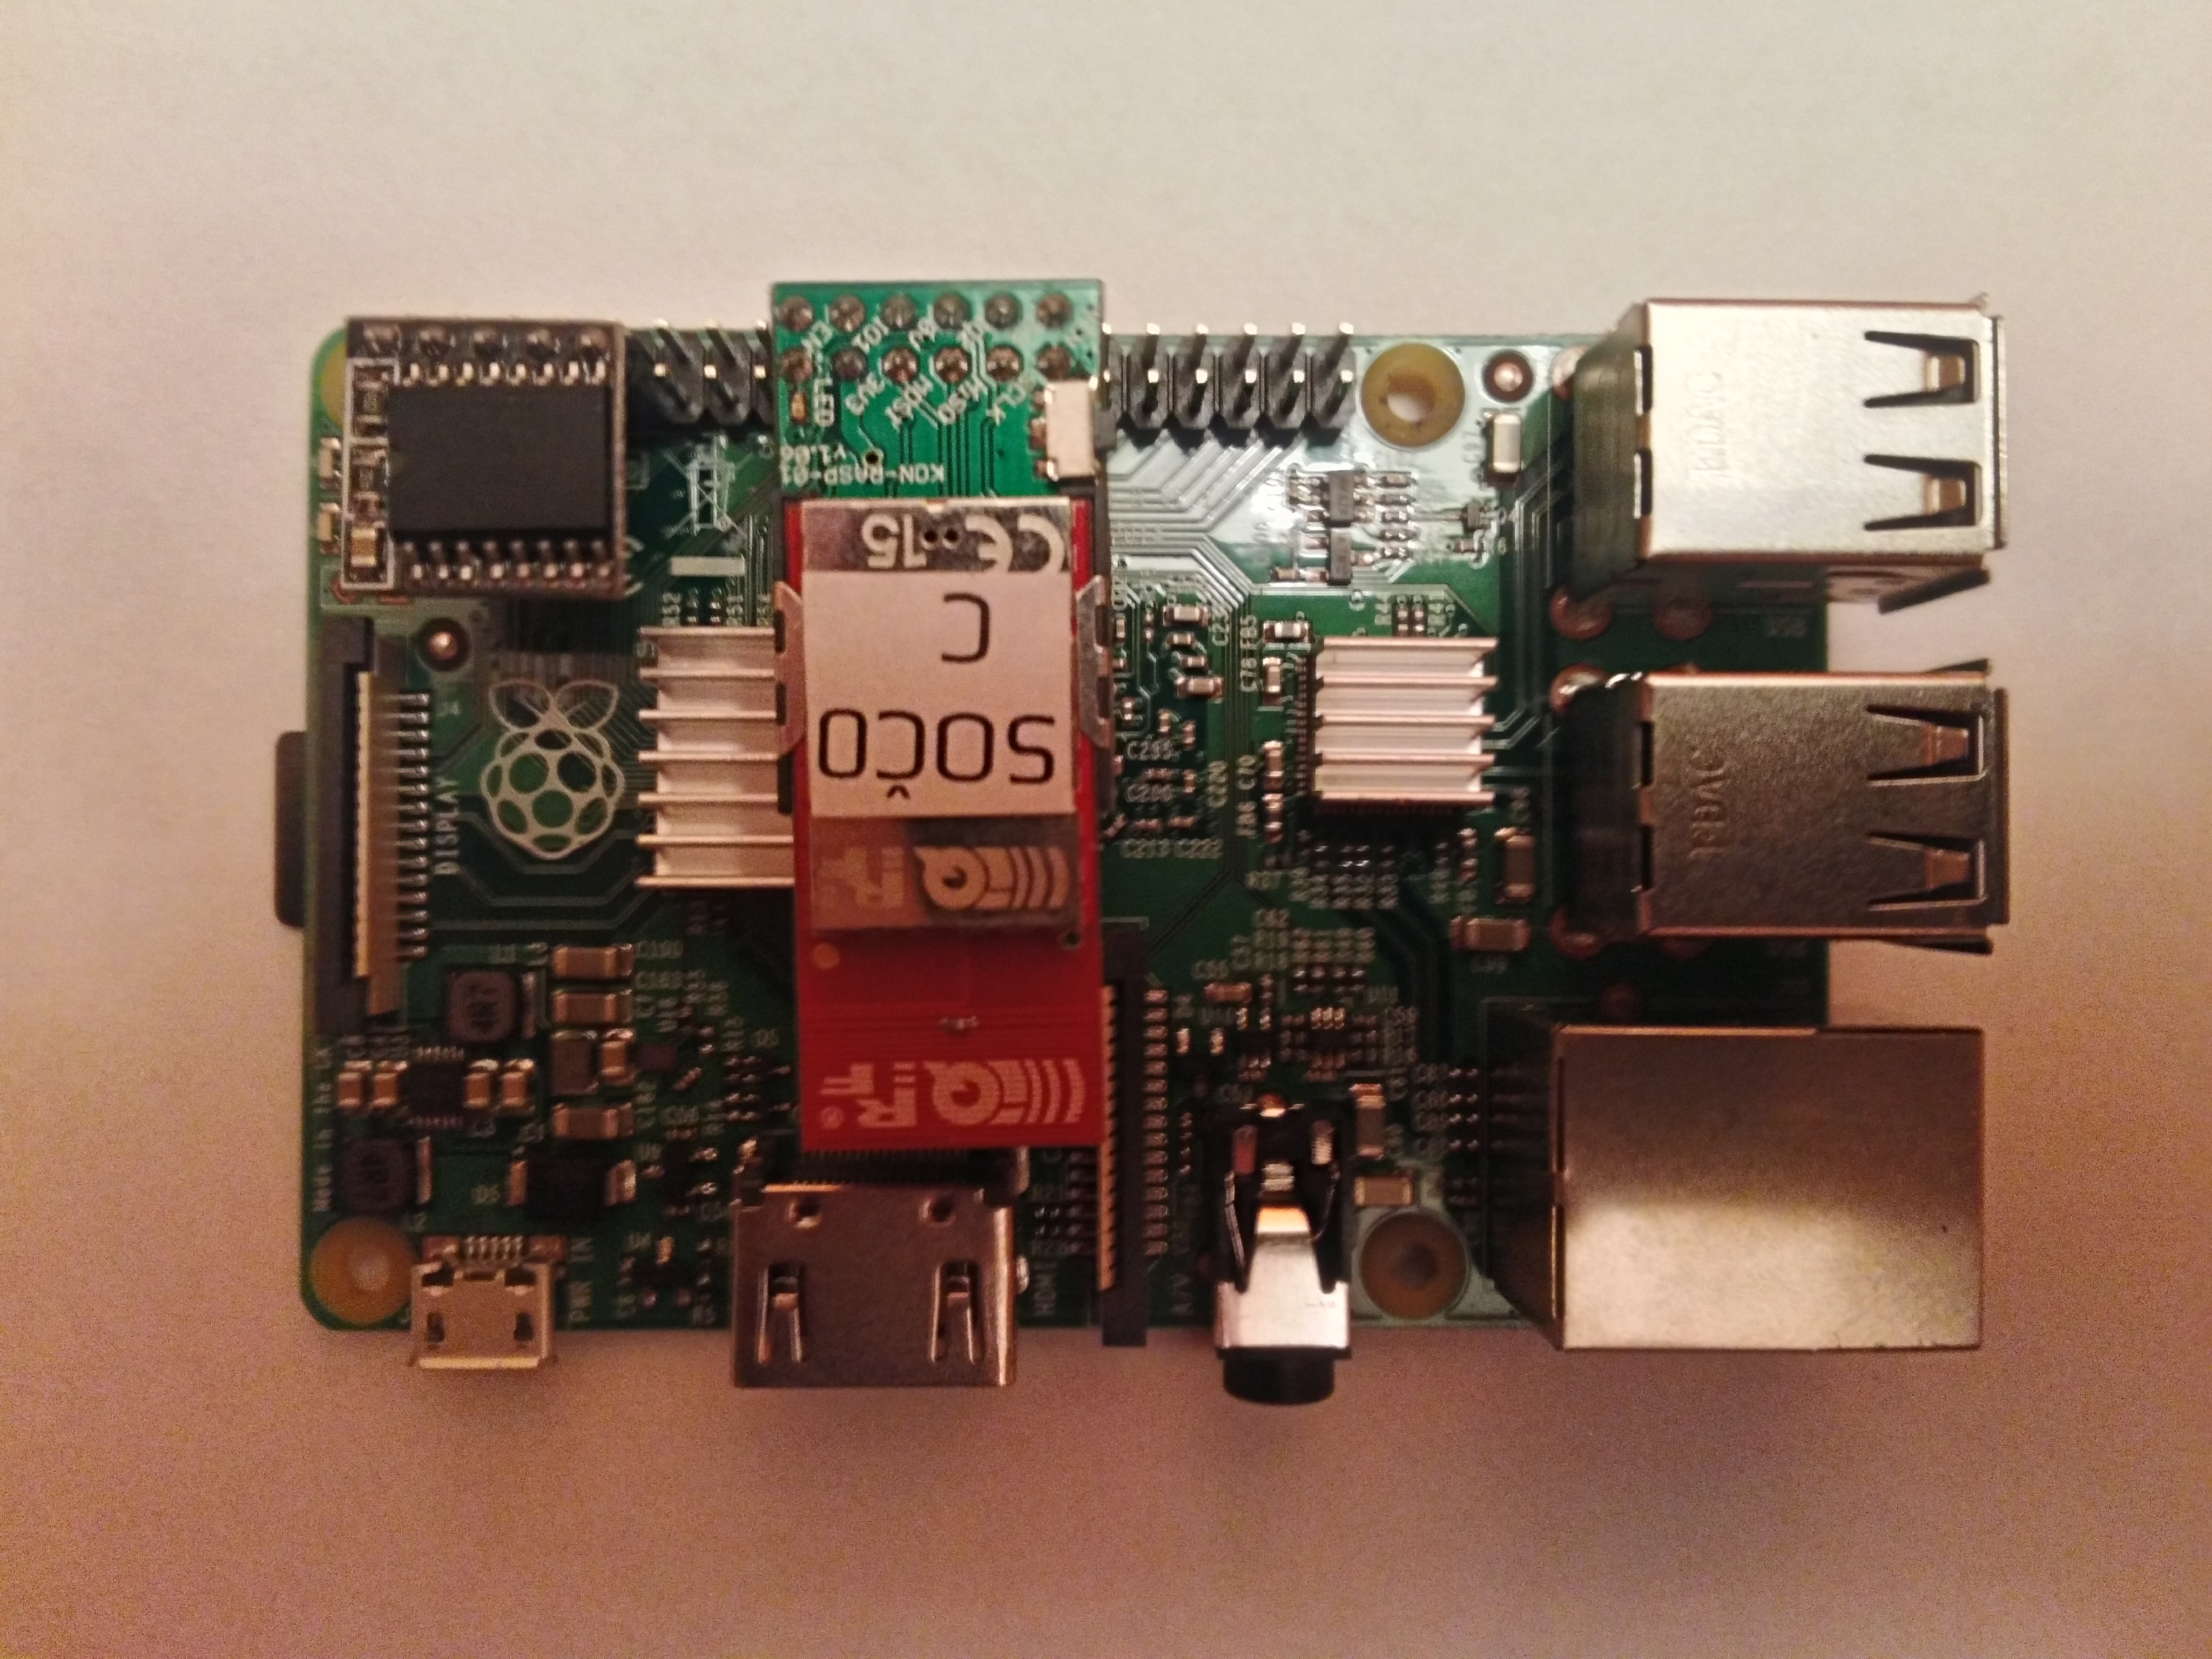
\includegraphics[width = 150mm]{img/foto/brana.jpg}
\caption{Fotografie funkčního vzorku brány}
\end{figure}

\begin{figure}[H]
\centering
\label{fig:foto/iqrf-pwm-fan-controller}
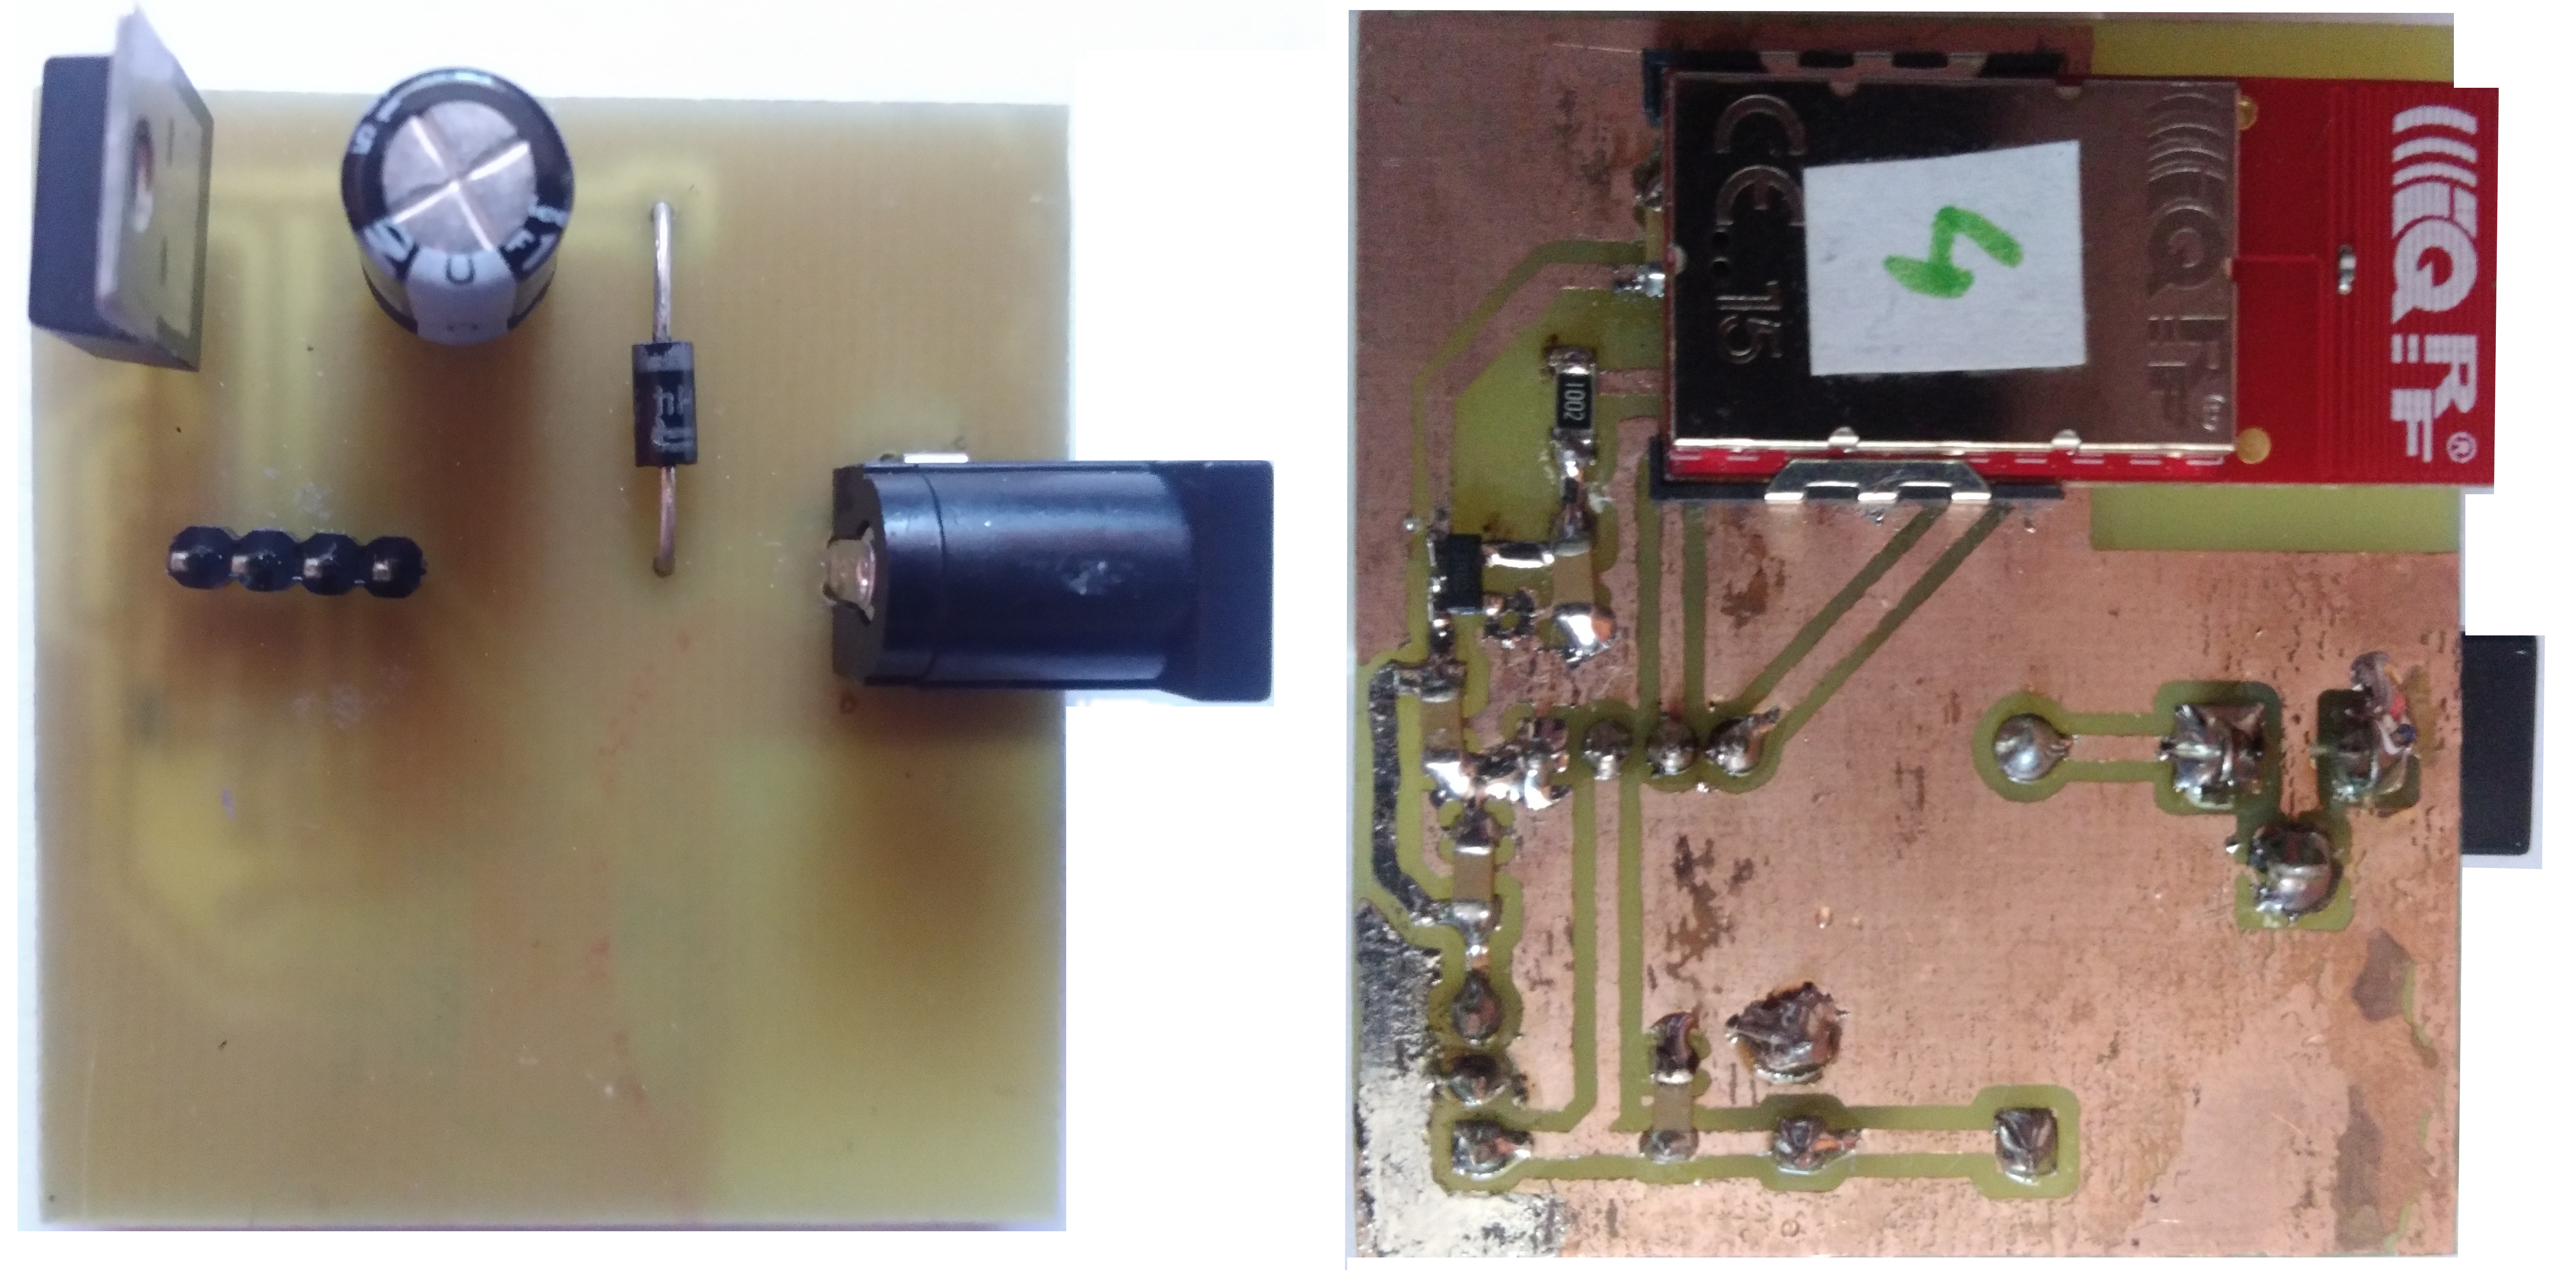
\includegraphics[width = 150mm]{img/foto/iqrf-pwm-fan-controller.jpg}
\caption{Fotografie funkčního vzorku PWM regulátor ventilátoru}
\end{figure}

\begin{figure}[H]
\centering
\label{fig:foto/arduino-ethernet-sensor}
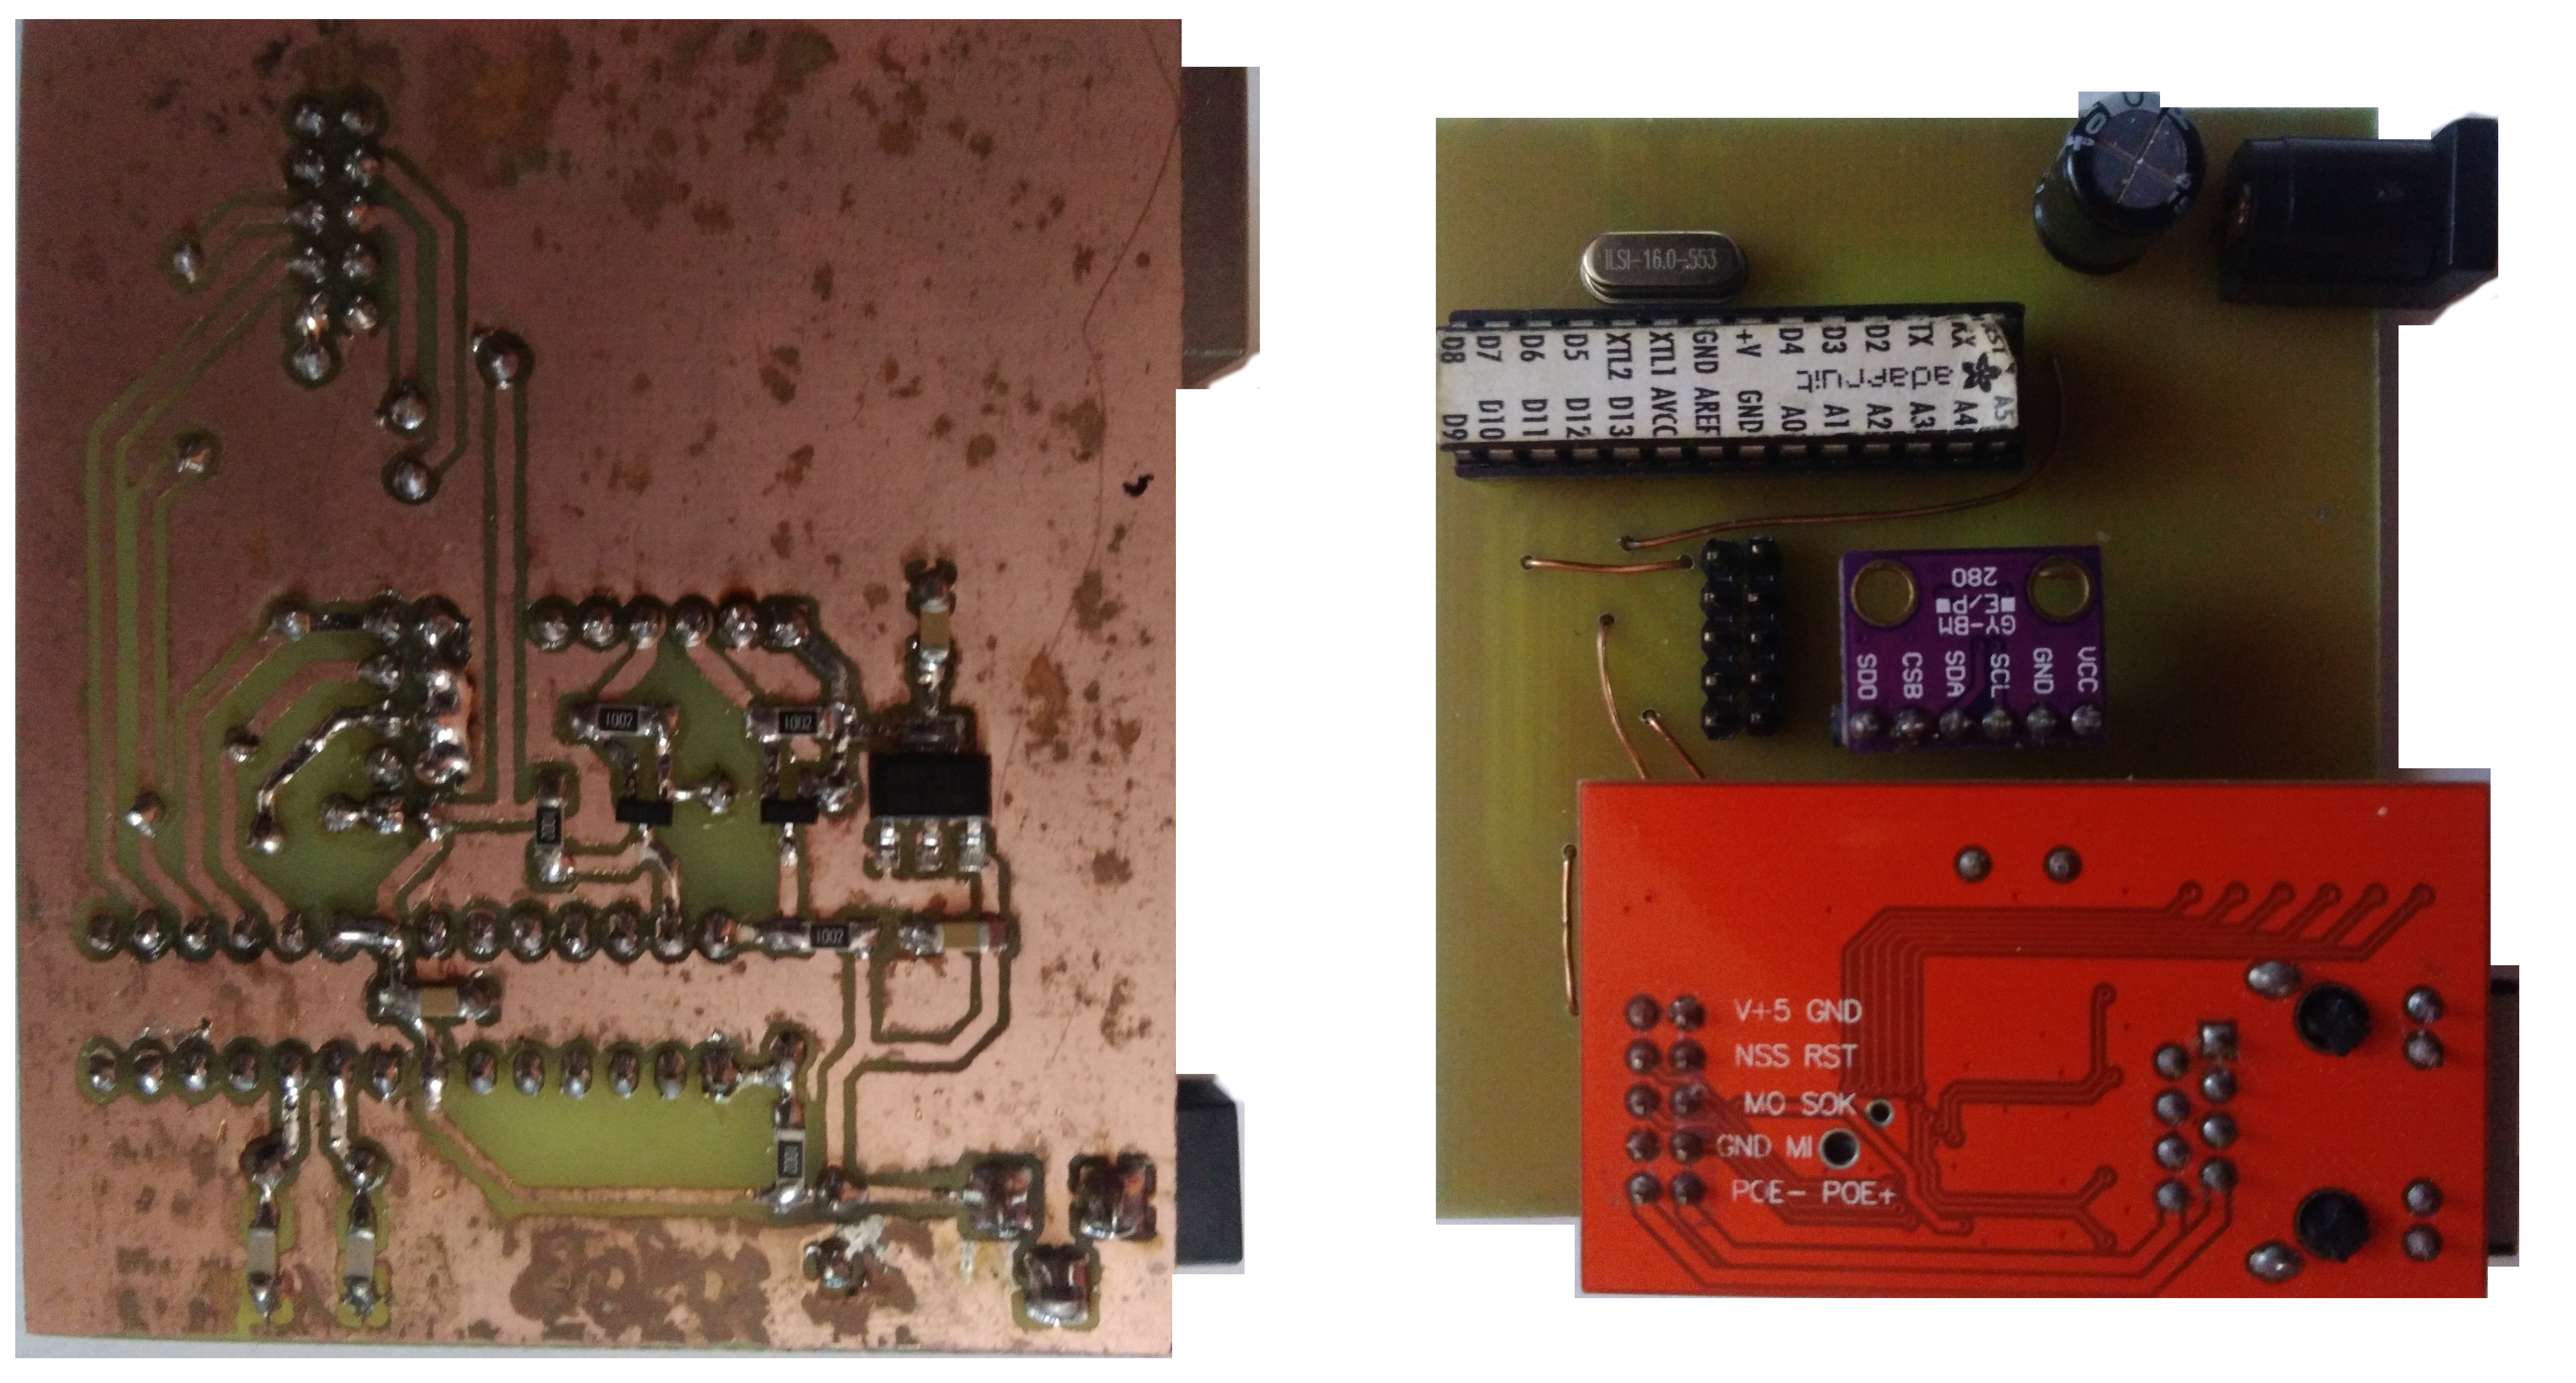
\includegraphics[width = 150mm]{img/foto/arduino-ethernet-sensor.jpg}
\caption{Fotografie funkčního vzorku senzoru teploty}
\end{figure}

\newpage

\printindex[zkr]

\addcontentsline{toc}{section}{Seznam použitých zkratek}

\newpage

\begin{thebibliography}{99}

\addcontentsline{toc}{section}{Seznam použité literatury}

\bibitem{bosch/bme280-datasheet}
Bosch Sensortec. BME280 Data sheet \emph{Bosch Sensortec} [online]. Jičín, 2018 [cit. 2018-04-08]. \\ Dostupné z: \url{https://www.iqrf.org/technology/iqrf-ide}

\bibitem{iqrf/ide}
IQRF Tech s.r.o. IQRF IDE \emph{IQRF} [online]. Jičín, 2018 [cit. 2018-04-08]. \\ Dostupné z: \url{https://www.iqrf.org/technology/iqrf-ide}

\bibitem{iqrf/os}
IQRF Tech s.r.o. Operating system \emph{IQRF} [online]. Jičín, 2018 [cit. 2018-04-08]. \\ Dostupné z: \url{https://www.iqrf.org/technology/operating-system}

\bibitem{iqrf/os/guide}
IQRF Tech s.r.o. IQRF OS v4.02D User's guide for TR-7xD \emph{IQRF} [online]. Jičín, 2017 [cit. 2018-04-08]. \\ Dostupné z: \url{http://www.iqrf.org/support/download&kat=35&ids=155}

\bibitem{iqrf/dpa}
IQRF Tech s.r.o. DPA \emph{IQRF} [online]. Jičín, 2018 [cit. 2018-04-08]. \\ Dostupné z: \url{https://www.iqrf.org/technology/dpa}

\bibitem{iqrf/dpa/guide}
IQRF Tech s.r.o. DPA Framework Technical guide v3.02 \emph{IQRF} [online]. Jičín, 2017 [cit. 2018-04-08]. \\ Dostupné z: \url{http://www.iqrf.org/support/download&kat=35&ids=155}

\bibitem{iqrf/dctr-72d-datasheet}
IQRF Tech s.r.o. Datasheet (DC)TR-72D \emph{IQRF} [online]. Jičín, 2017 [cit. 2018-04-08]. \\ Dostupné z: \url{http://iqrf.org/weben/downloads.php?id=337}

\bibitem{iqrf/kon-rasp-01-datasheet}
IQRF Tech s.r.o. User's guide KON-RASP-01 \emph{IQRF} [online]. Jičín, 2015 [cit. 2018-04-08]. \\ Dostupné z: \url{http://www.iqrf.org/weben/downloads.php?id=412}

\bibitem{iqrfsdk/iqrf-daemon}
IQRF Tech s.r.o. IQRF Gateway Daemon \emph{IQRF} [online]. Jičín, 2018 [cit. 2018-04-08]. \\ Dostupné z: \url{https://github.com/iqrfsdk/iqrf-daemon}

\bibitem{iqrfsdk/iqrf-daemon-webapp}
IQRF Tech s.r.o. IQRF Gateway Daemon webapp \emph{IQRF} [online]. Jičín, 2018 [cit. 2018-04-08]. \\ Dostupné z: \url{https://github.com/iqrfsdk/iqrf-daemon-webapp}

\bibitem{nette}
Nette Foundation. Nette Framework \emph{Nette} [online]. Praha, 2018 [cit. 2018-04-08]. \\ Dostupné z: \url{https://nette.org/}

\bibitem{microchip/atmega328p-datasheet}
Microchip. ATmega328/P AVR MCU with picoPower Technology Data Sheet \emph{Microchip} [online]. 2018 [cit. 2018-04-08]. \\ Dostupné z: \url{http://ww1.microchip.com/downloads/en/DeviceDoc/ATmega328_P%20AVR%20MCU%20with%20picoPower%20Technology%20Data%20Sheet%2040001984A.pdf}

\bibitem{microchip/pic16f1938}
Microchip. PIC16F1938 \emph{PIC16F1938} [online]. 2017 [cit. 2018-04-08]. \\ Dostupné z: \url{http://www.microchip.com/wwwproducts/en/PIC16F1938}

\bibitem{rpi3-spec}
Raspberry Pi Foundation. Raspberry Pi 3 Model B Specifications \emph{Raspberry Pi} [online]. UK, 2018 [cit. 2018-04-08]. \\ Dostupné z: \url{https://www.raspberrypi.org/products/raspberry-pi-3-model-b/}

\bibitem{sw/atom}
GitHub. Atom \emph{Atom} [online]. 2018 [cit. 2018-04-08]. \\ Dostupné z: \url{https://atom.io/}

\bibitem{sw/cc5x-compiler}
B Knudsen Data. CC5X C Compiler \emph{CC5X} [online]. Norsko, 2017 [cit. 2018-04-08]. \\ Dostupné z: \url{http://www.bknd.com/cc5x/}

\bibitem{sw/dia}
Gnome. Dia \emph{Dia} [online]. 2018 [cit. 2018-04-08]. \\ Dostupné z: \url{https://wiki.gnome.org/Apps/Dia/}

\bibitem{sw/kicad}
KiCad EDA\index[zkr]{EDA!Electronic design automation|textit} \emph{KiCad EDA} [online]. 2018 [cit. 2018-04-08]. \\ Dostupné z: \url{http://kicad-pcb.org/}

\bibitem{sw/mosquitto}
Eclipse Foundation. Eclipse Mosquitto \emph{Eclipse} [online]. 2018 [cit. 2018-04-08]. \\ Dostupné z: \url{https://mosquitto.org/}

\bibitem{sw/node-red}
Node-RED \emph{Node-RED} [online]. 2018 [cit. 2018-04-08]. \\ Dostupné z: \url{https://nodered.org/}

\bibitem{sw/platformio-ide}
PlatormIO. PlatformIO IDE \emph{PlatformIO} [online]. 2018 [cit. 2018-04-08]. \\ Dostupné z: \url{https://platformio.org/platformio-ide}

\bibitem{wiki/ism-band}
Wikipedia. ISM\index[zkr]{ISM!Industrial, Scientific and Medical|textit} Band \emph{Wikipedia} [online]. [cit. 2018-04-08]. \\ Dostupné z: \url{https://en.wikipedia.org/wiki/ISM\_band}

\bibitem{wiki/node-red}
Wikipedia. Node-RED \emph{Wikipedia} [online]. [cit. 2018-04-08]. \\ Dostupné z: \url{https://en.wikipedia.org/wiki/Node-RED}

\bibitem{wiznet/w5100}
WIZnet Co., Inc. W5100 Datasheet \emph{WIZnet} [online]. 2011 [cit. 2018-04-08]. \\ Dostupné z: \url{http://www.wiznet.io/wp-content/uploads/wiznethome/Chip/W5100/Document/W5100_Datasheet_v1.2.7.pdf}

\end{thebibliography}

\newpage

\listoffigures

\addcontentsline{toc}{section}{Seznam obrázků}

\listoftables

\addcontentsline{toc}{section}{Seznam tabulek}

\end{document}
